% \begin{figure*}[t!]
% 	% \vspace{-20pt}
% 	\centering
% 	\resizebox{0.98\linewidth}{!}{
% 	\renewcommand{\arraystretch}{0.5}
% 	\begin{tabular}{@{}c@{\hskip 0.05cm}c@{\hskip 0.05cm}c@{\hskip 0.05cm}c@{\hskip 0.05cm}c@{\hskip 0.05cm}c@{}}
% 		\centering
%             &
% 		{\small Input $t_0$}&
% 		{\small Tracked $t_0$}&
% 		{\small Tracked $t_1$}&
% 		{\small Tracked $t_2$}&
% 		{\small Tracked $t_3$}\\

%             \rotatebox[origin=c]{90}{{\footnotesize	  Suburban}}&
% 		 \raisebox{-0.5\height}{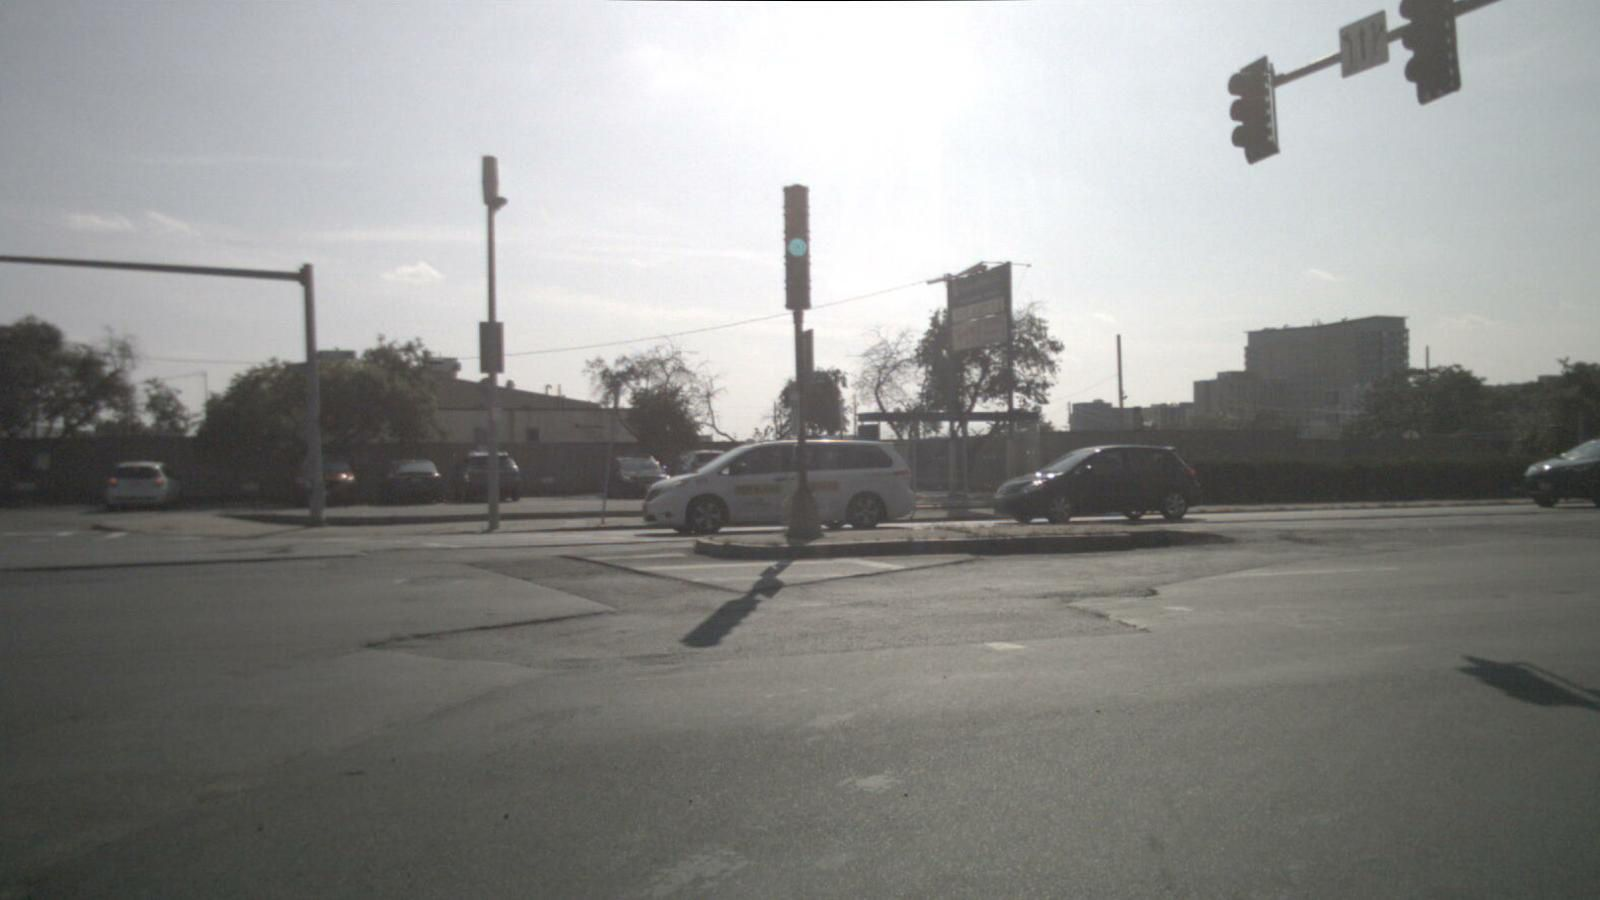
\includegraphics[width=.19\columnwidth, trim={0cm 0cm 0cm 0cm},clip]{fig/nuScenes_main/scene2/0484_2_gt.png}}&
% 		 \raisebox{-0.5\height}{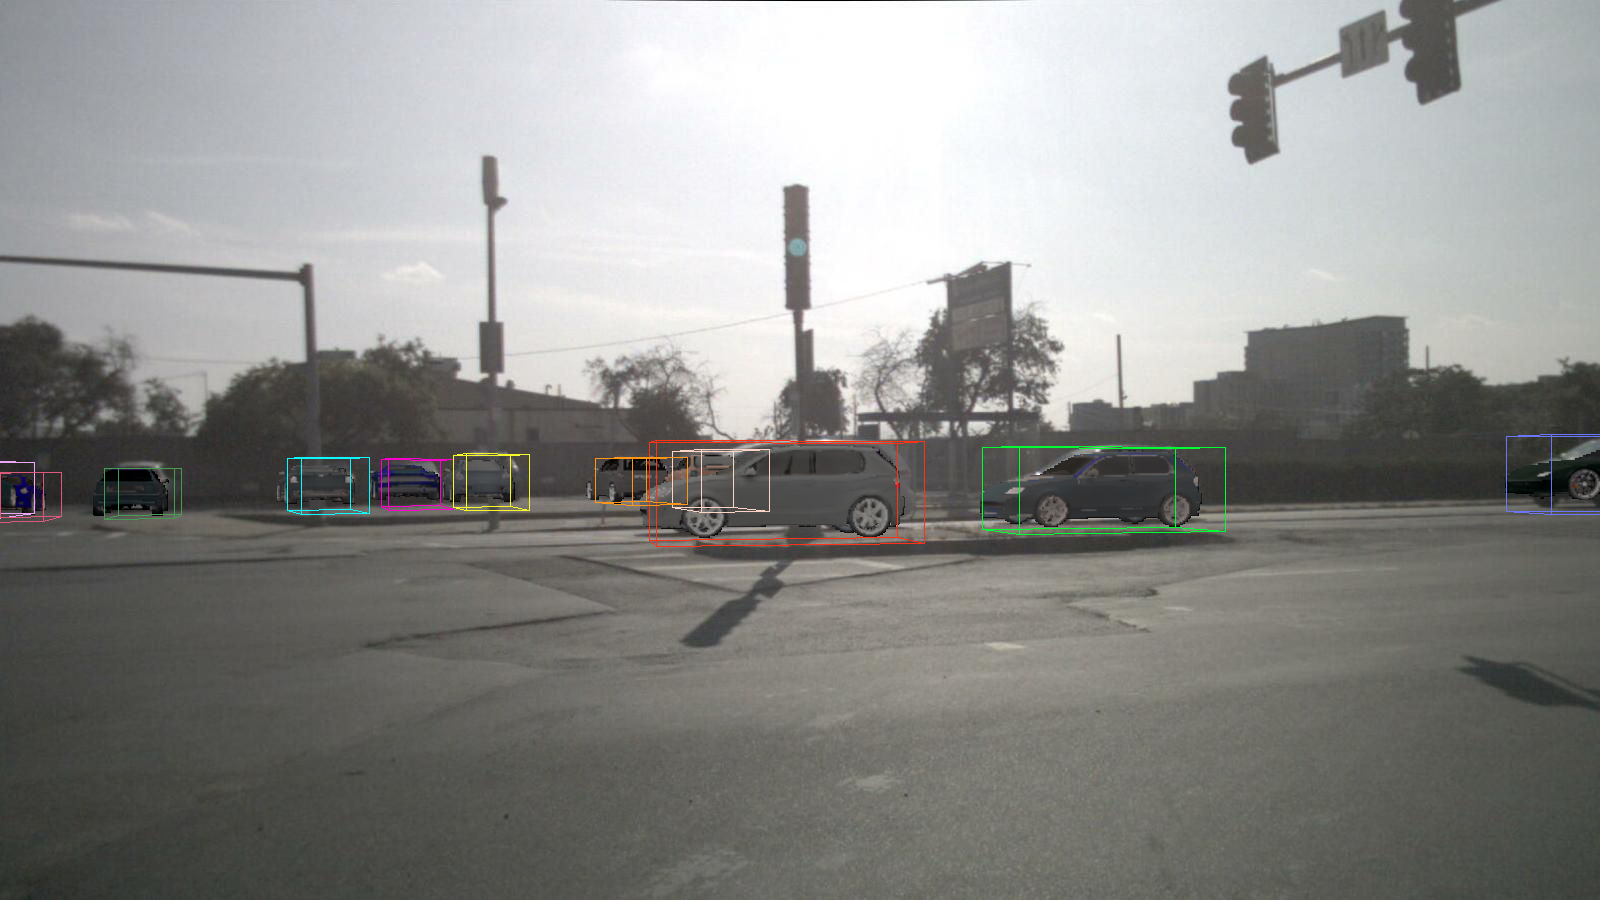
\includegraphics[width=.19\columnwidth, trim={0cm 0cm 0cm 0cm},clip]{fig/nuScenes_main/scene2/0484_2_bbox.png}}&
% 		 \raisebox{-0.5\height}{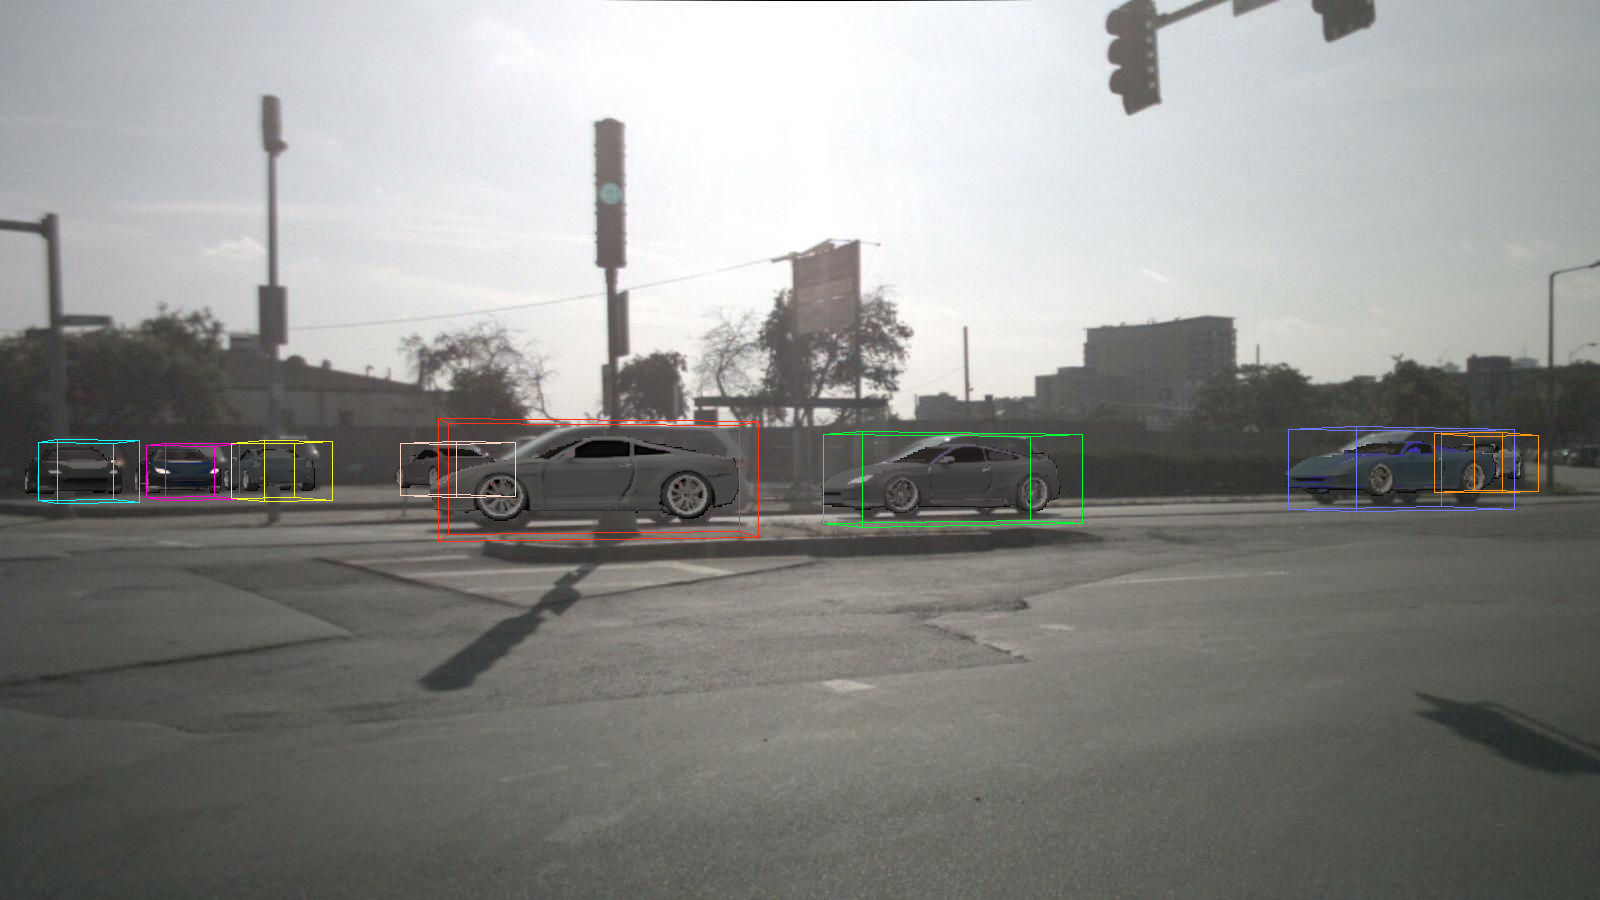
\includegraphics[width=.19\columnwidth, trim={0cm 0cm 0cm 0cm},clip]{fig/nuScenes_main/scene2/0484_3_bbox.png}}&
% 		 \raisebox{-0.5\height}{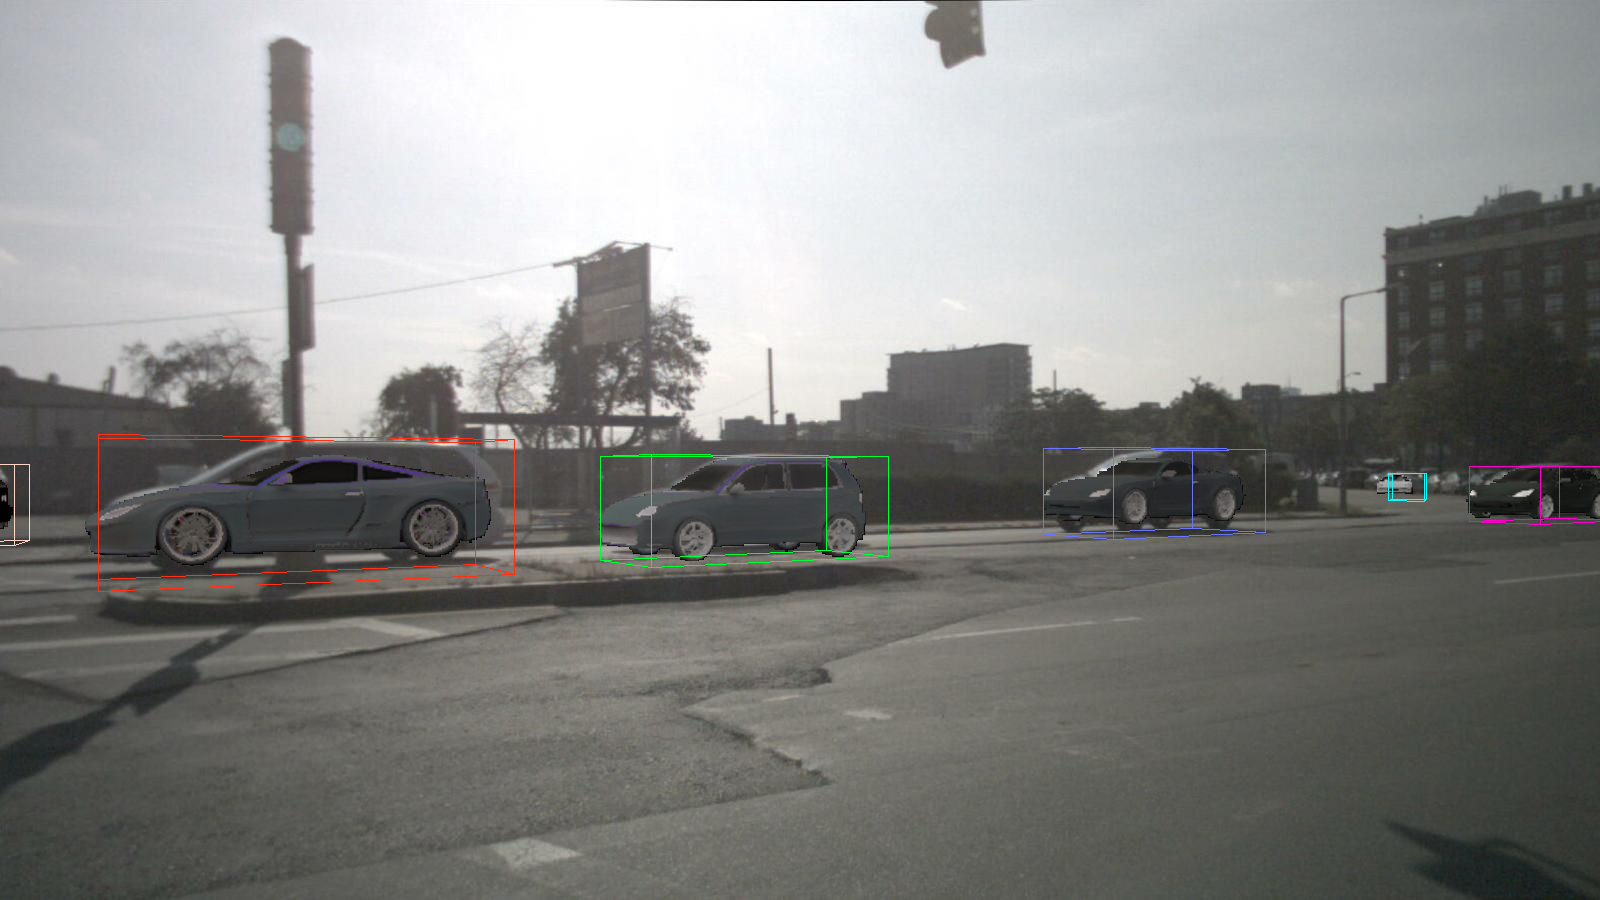
\includegraphics[width=.19\columnwidth, trim={0cm 0cm 0cm 0cm},clip]{fig/nuScenes_main/scene2/0484_4_bbox.png}}&
% 		 \raisebox{-0.5\height}{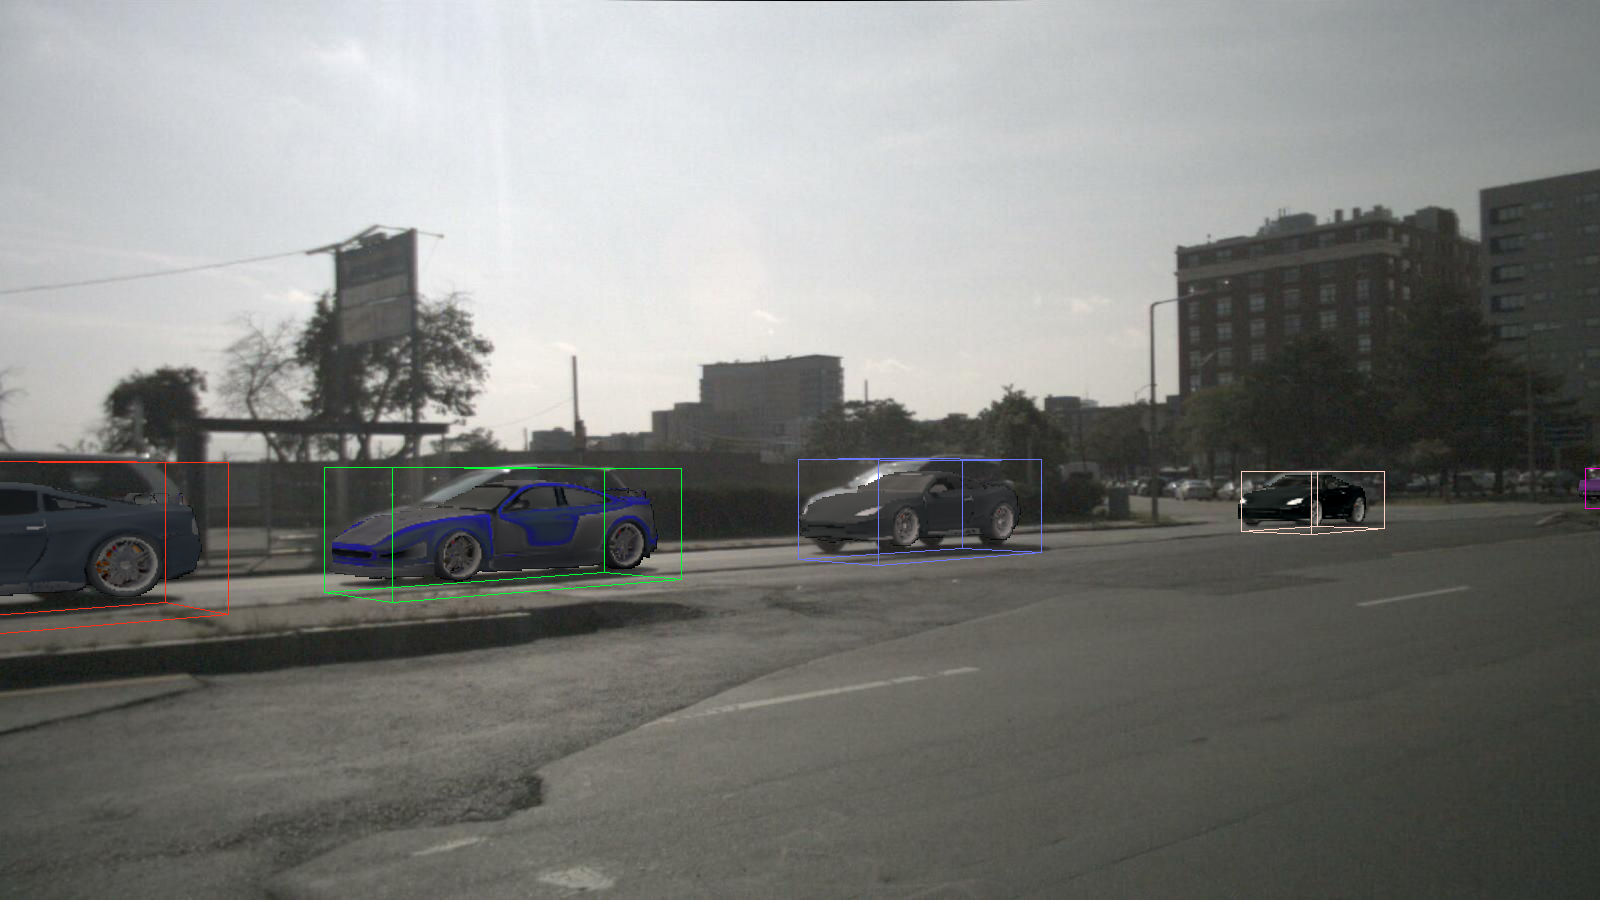
\includegraphics[width=.19\columnwidth, trim={0cm 0cm 0cm 0cm},clip]{fig/nuScenes_main/scene2/0484_5_bbox.png}}\\[0.95cm]
  
% 		\rotatebox[origin=c]{90}{{\footnotesize	 Dense Urban}}&
% 		\raisebox{-0.5\height}{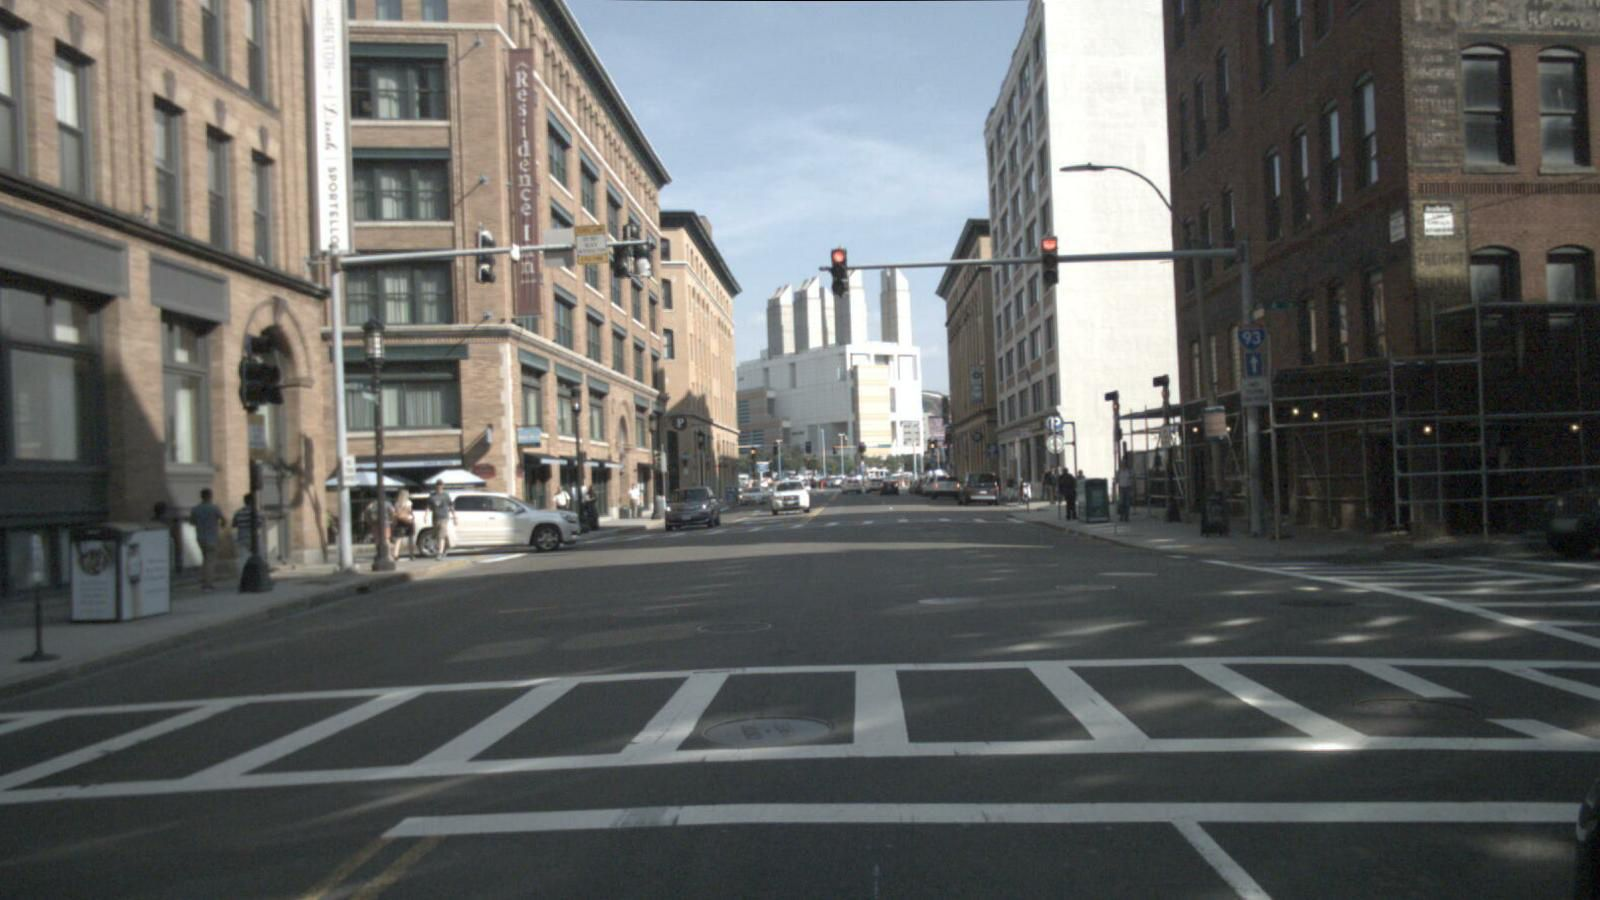
\includegraphics[width=.19\columnwidth, trim={0cm 0cm 0cm 0cm},clip]{fig/nuScenes_main/scene3/0496_30_gt.png}}&
% 		\raisebox{-0.5\height}{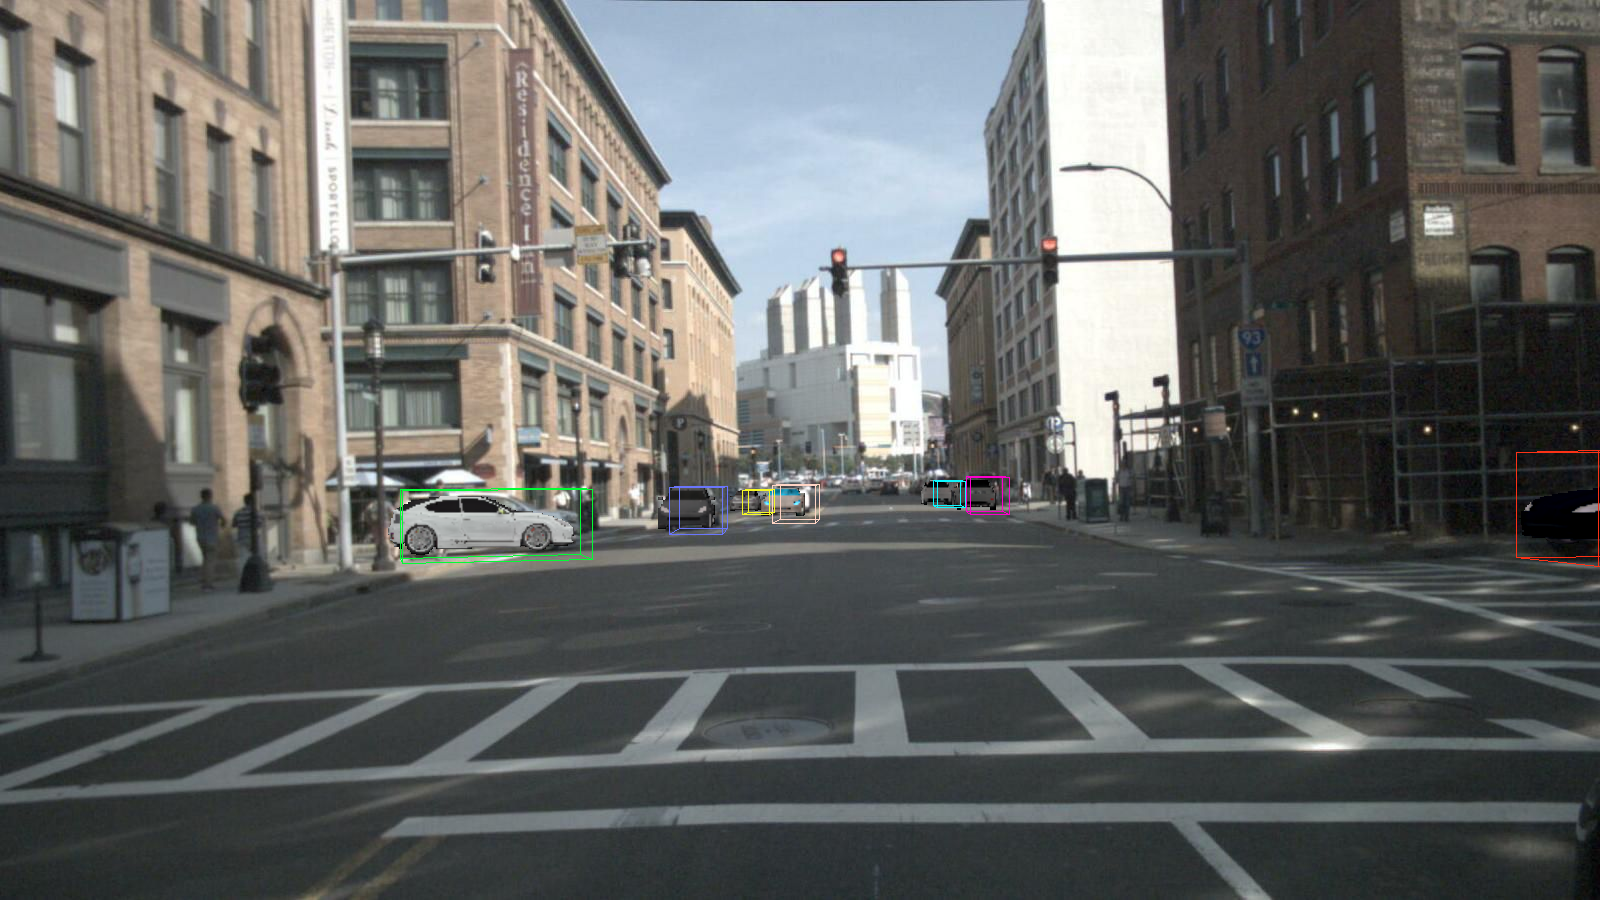
\includegraphics[width=.19\columnwidth, trim={0cm 0cm 0cm 0cm},clip]{fig/nuScenes_main/scene3/0496_30_bbox.png}} &
% 		\raisebox{-0.5\height}{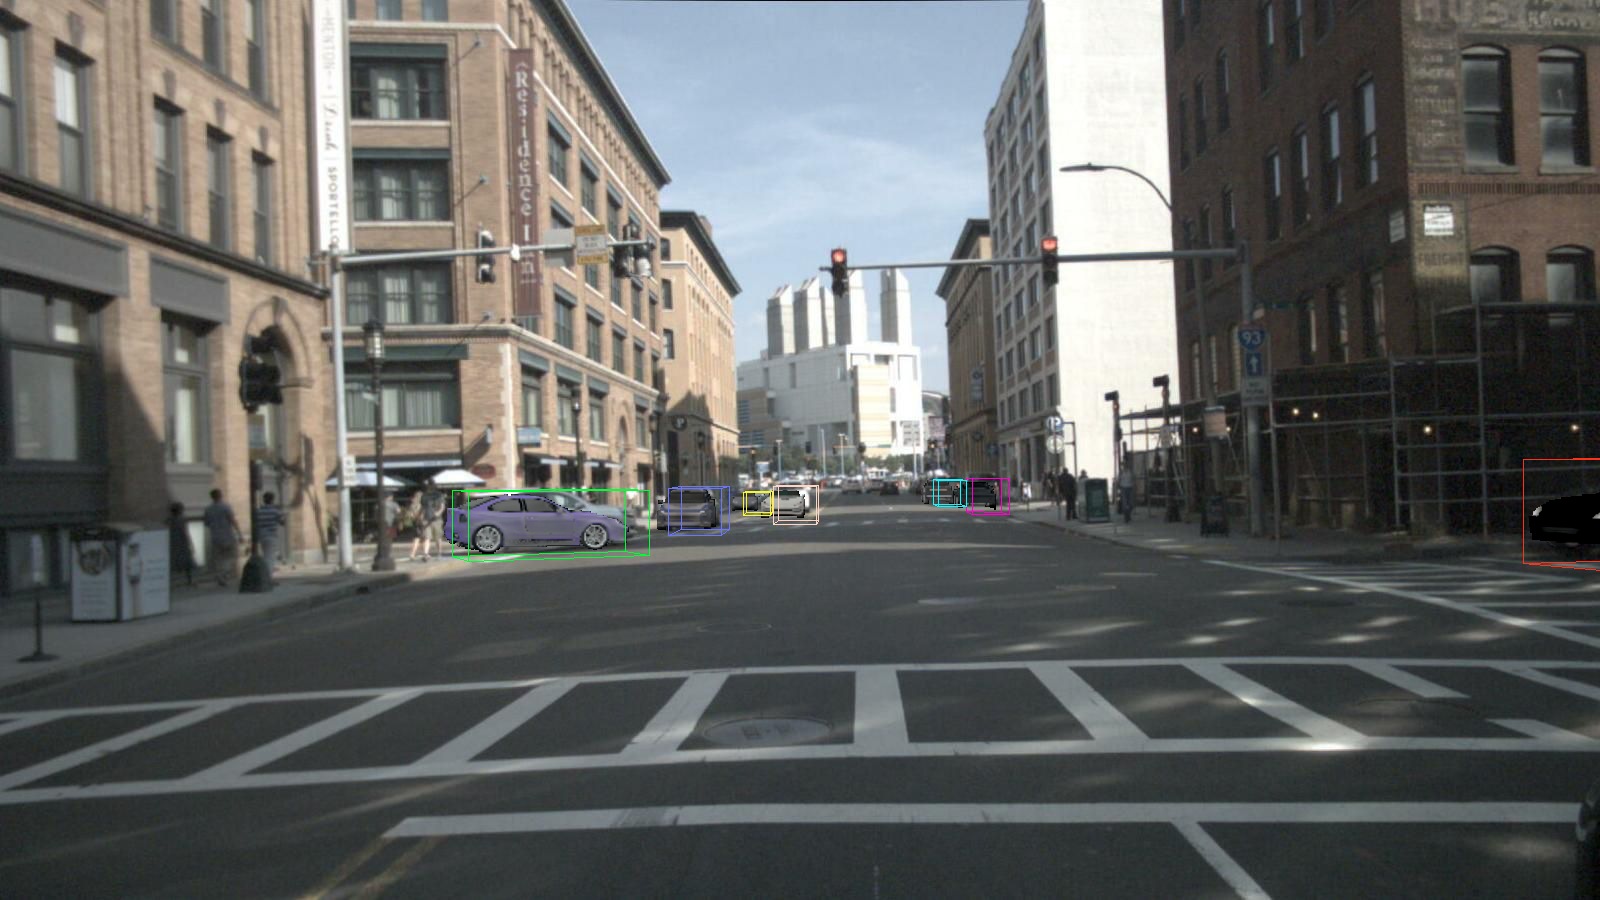
\includegraphics[width=.19\columnwidth, trim={0cm 0cm 0cm 0cm},clip]{fig/nuScenes_main/scene3/0496_31_bbox.png}}&
% 		\raisebox{-0.5\height}{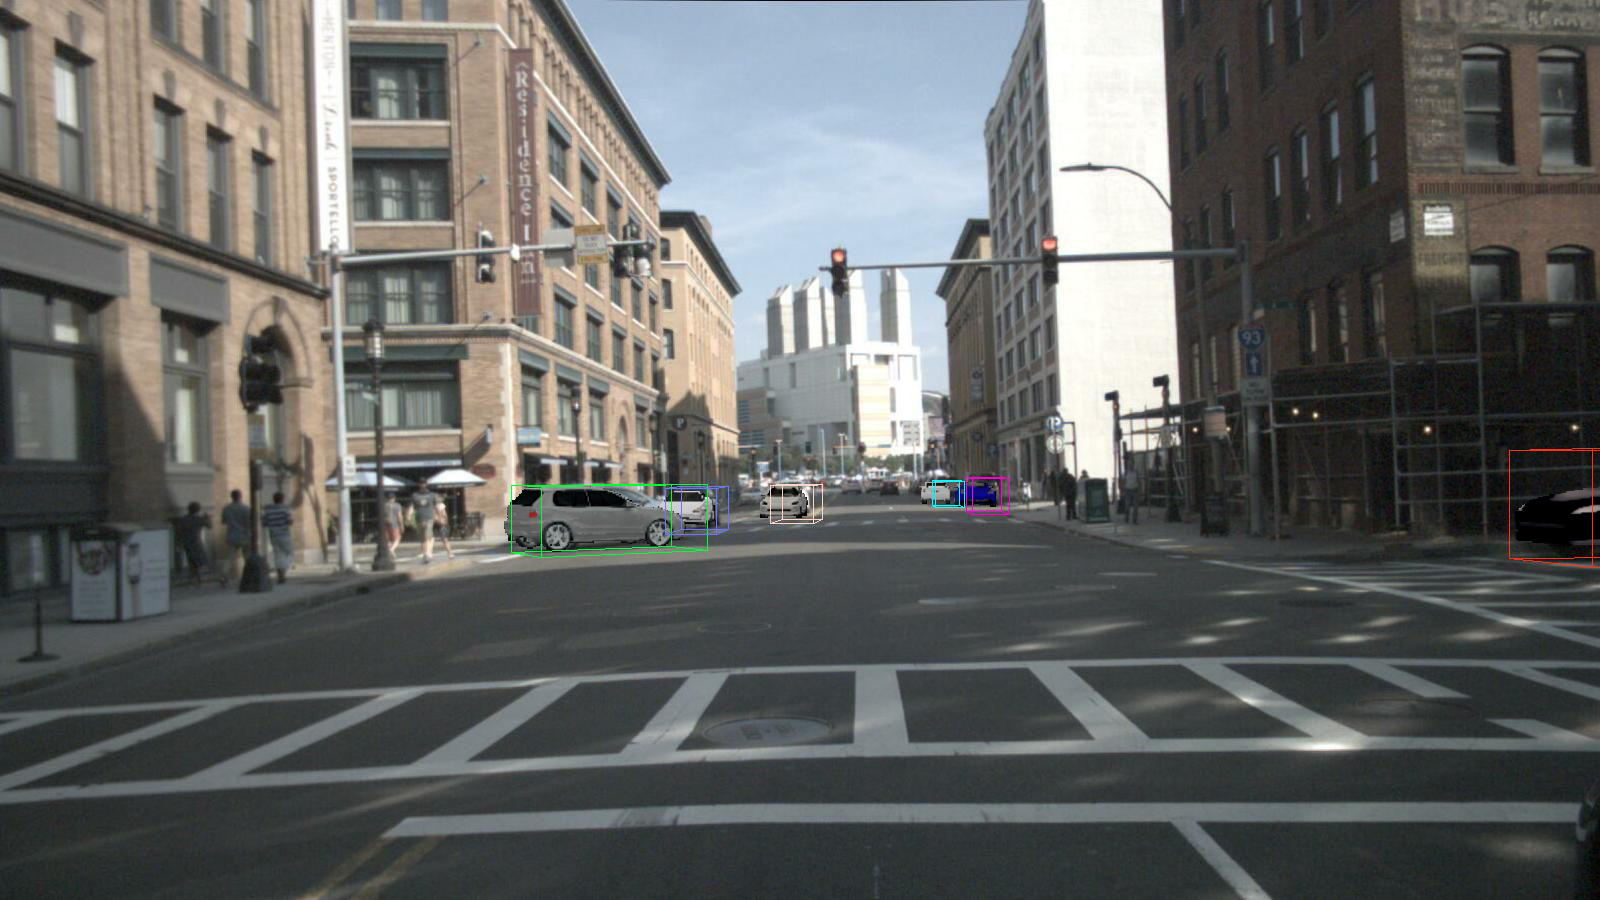
\includegraphics[width=.19\columnwidth, trim={0cm 0cm 0cm 0cm},clip]{fig/nuScenes_main/scene3/0496_32_bbox.png}}&
% 		\raisebox{-0.5\height}{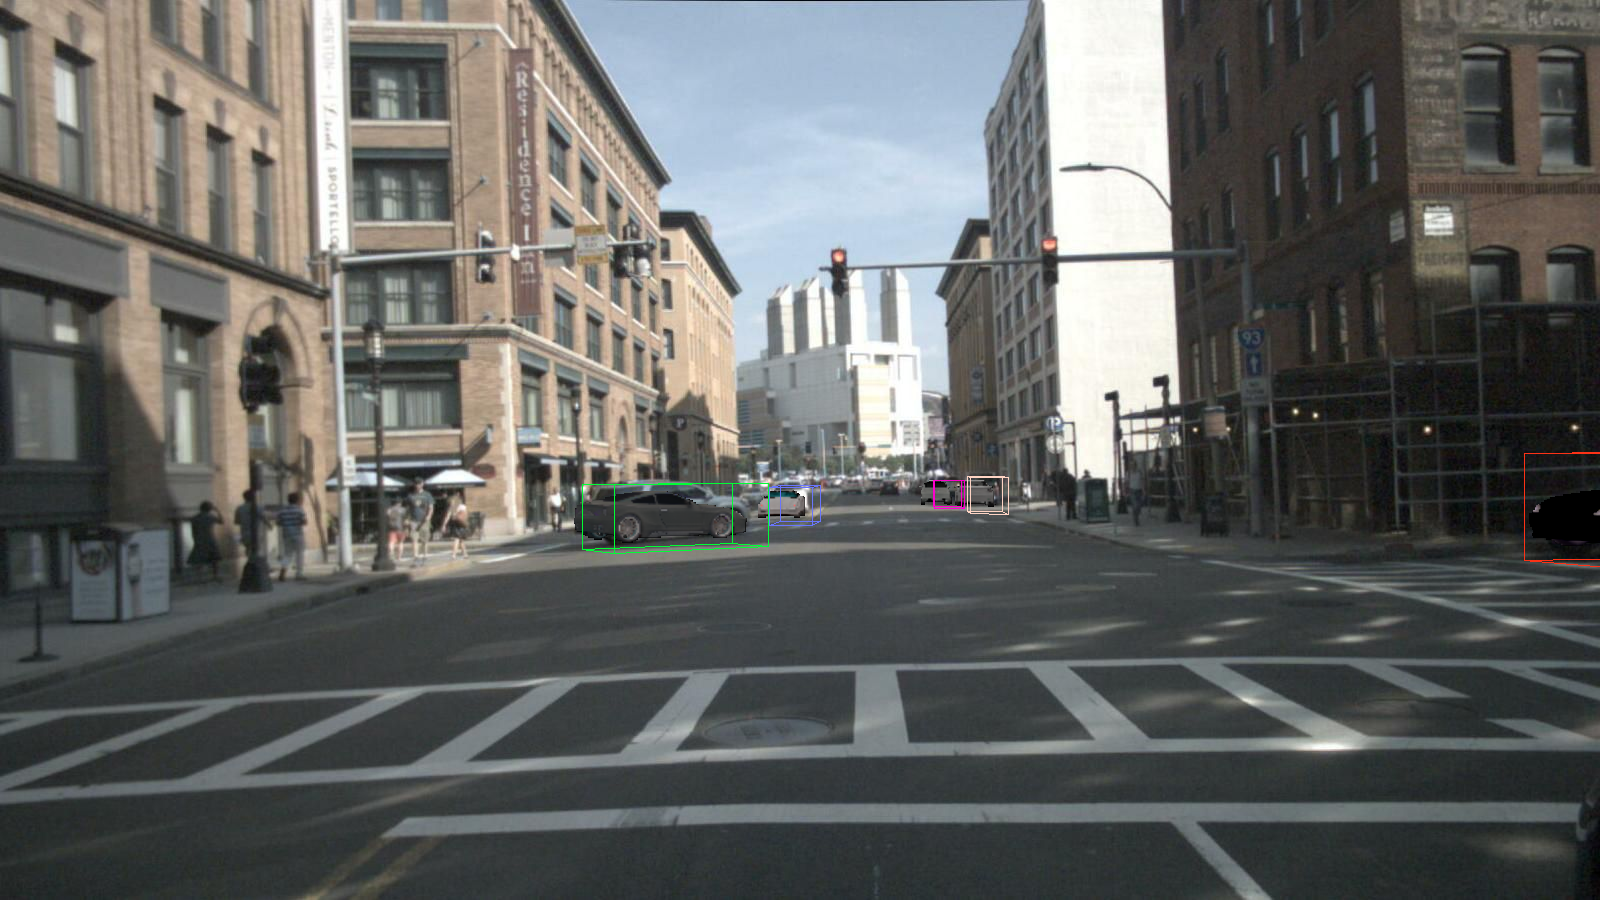
\includegraphics[width=.19\columnwidth, trim={0cm 0cm 0cm 0cm},clip]{fig/nuScenes_main/scene3/0496_33_bbox.png}}\\[0.7cm]
  
%             \rotatebox[origin=c]{90}{{\footnotesize	 Clutter}}&
%   		\raisebox{-0.5\height}{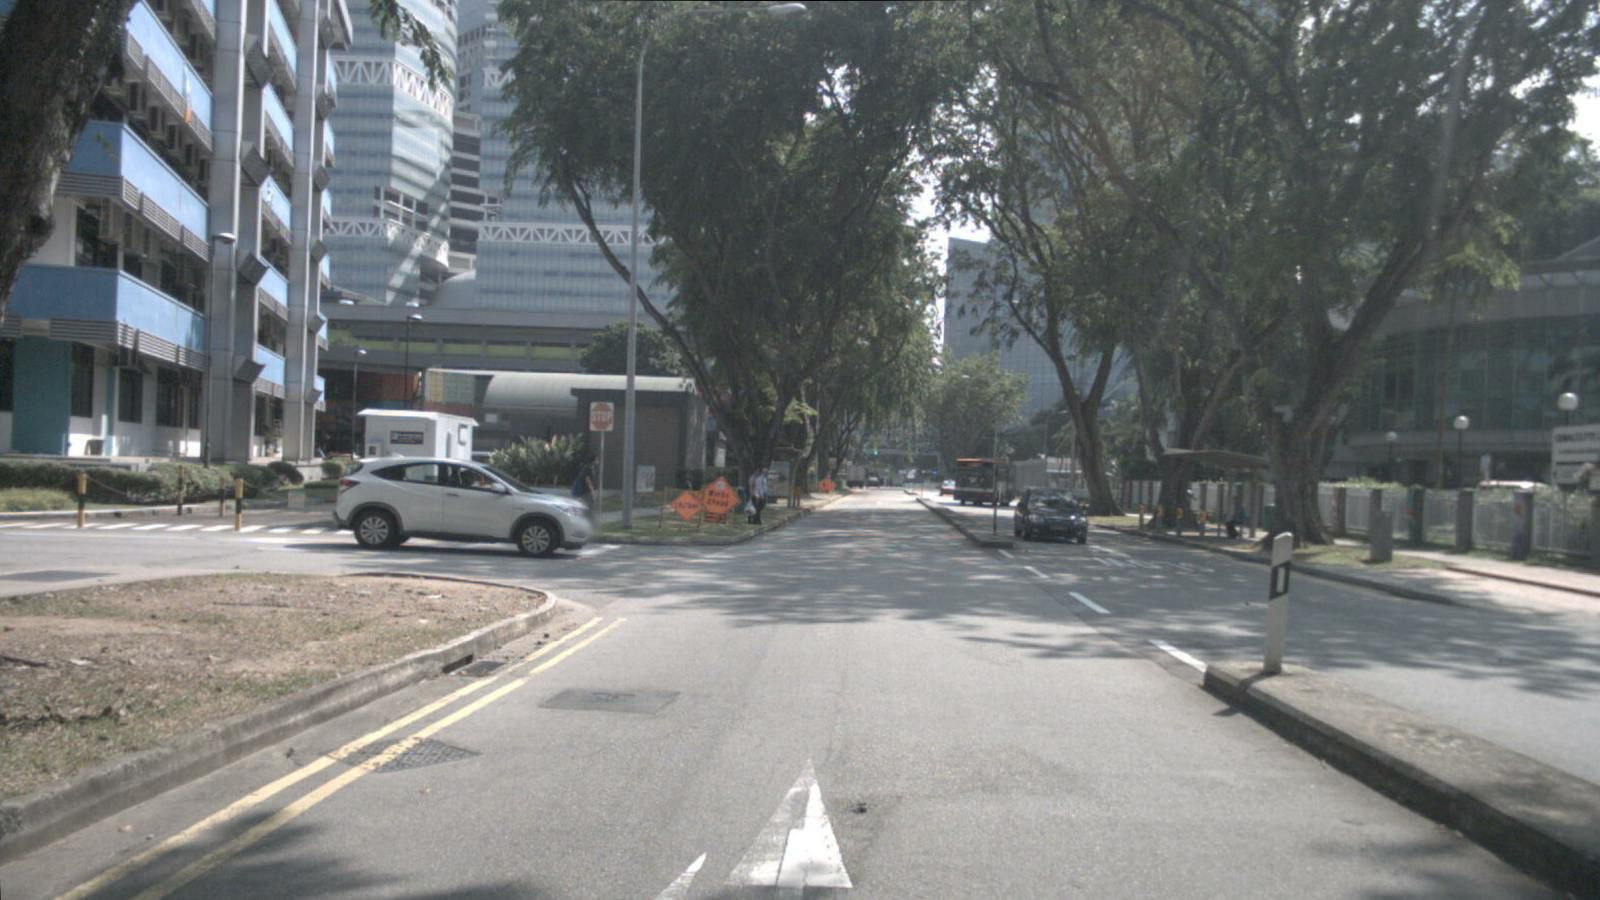
\includegraphics[width=.19\columnwidth, trim={0cm 0cm 0cm 0cm},clip]{fig/nuScenes_main/scene6/28_gt_img.png}}&
% 		\raisebox{-0.5\height}{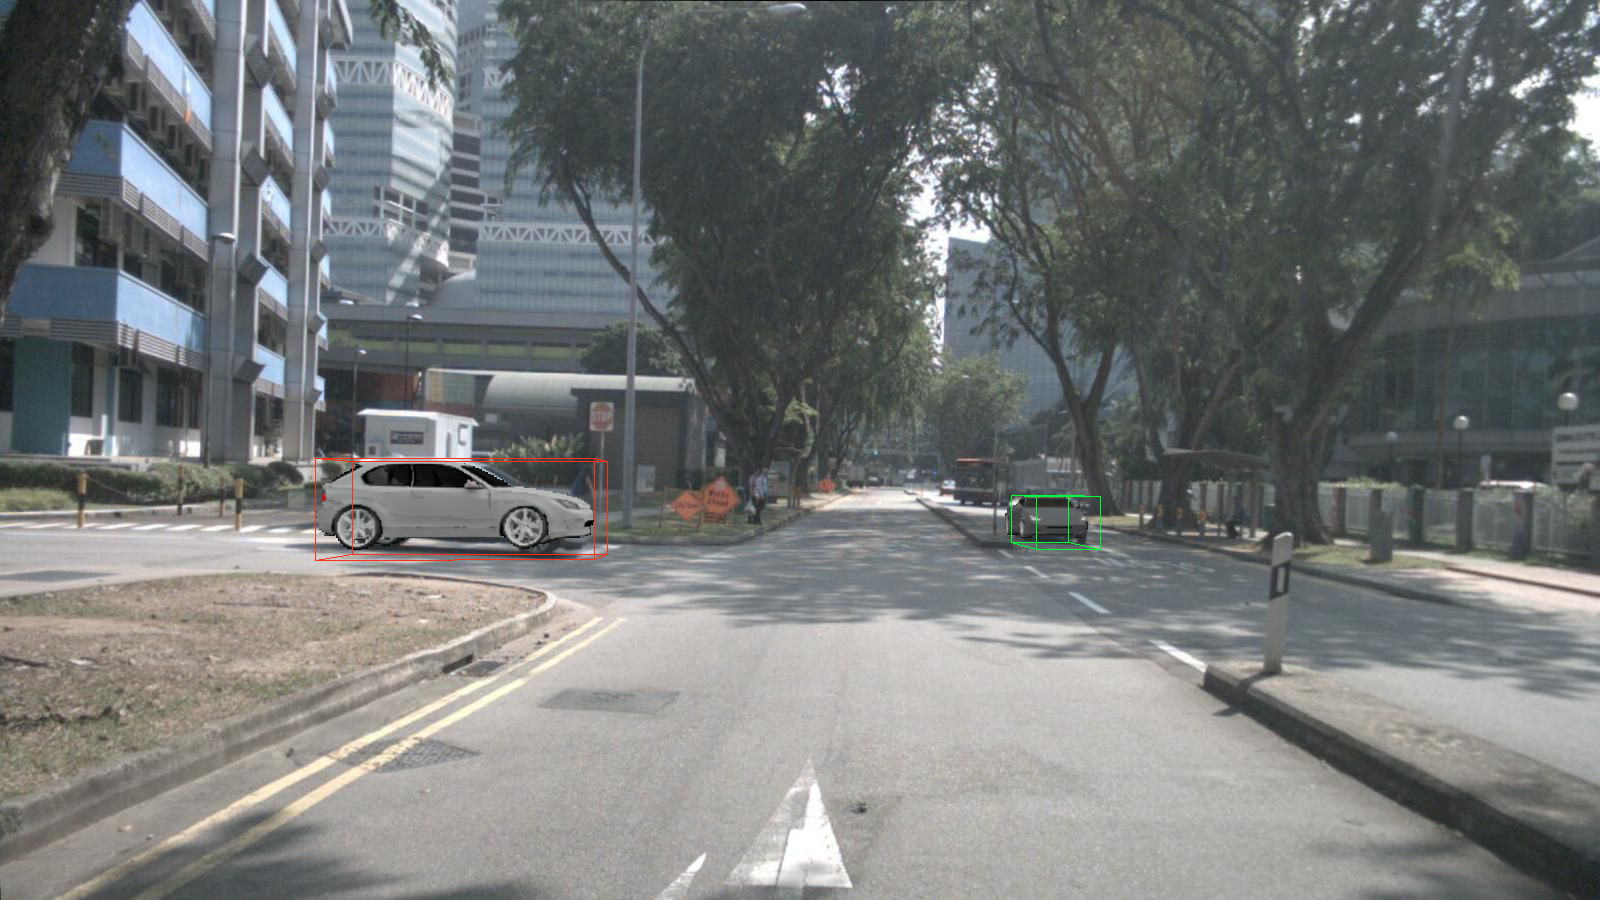
\includegraphics[width=.19\columnwidth, trim={0cm 0cm 0cm 0cm},clip]{fig/nuScenes_main/scene6/35_28_bbox.png}}&
% 		\raisebox{-0.5\height}{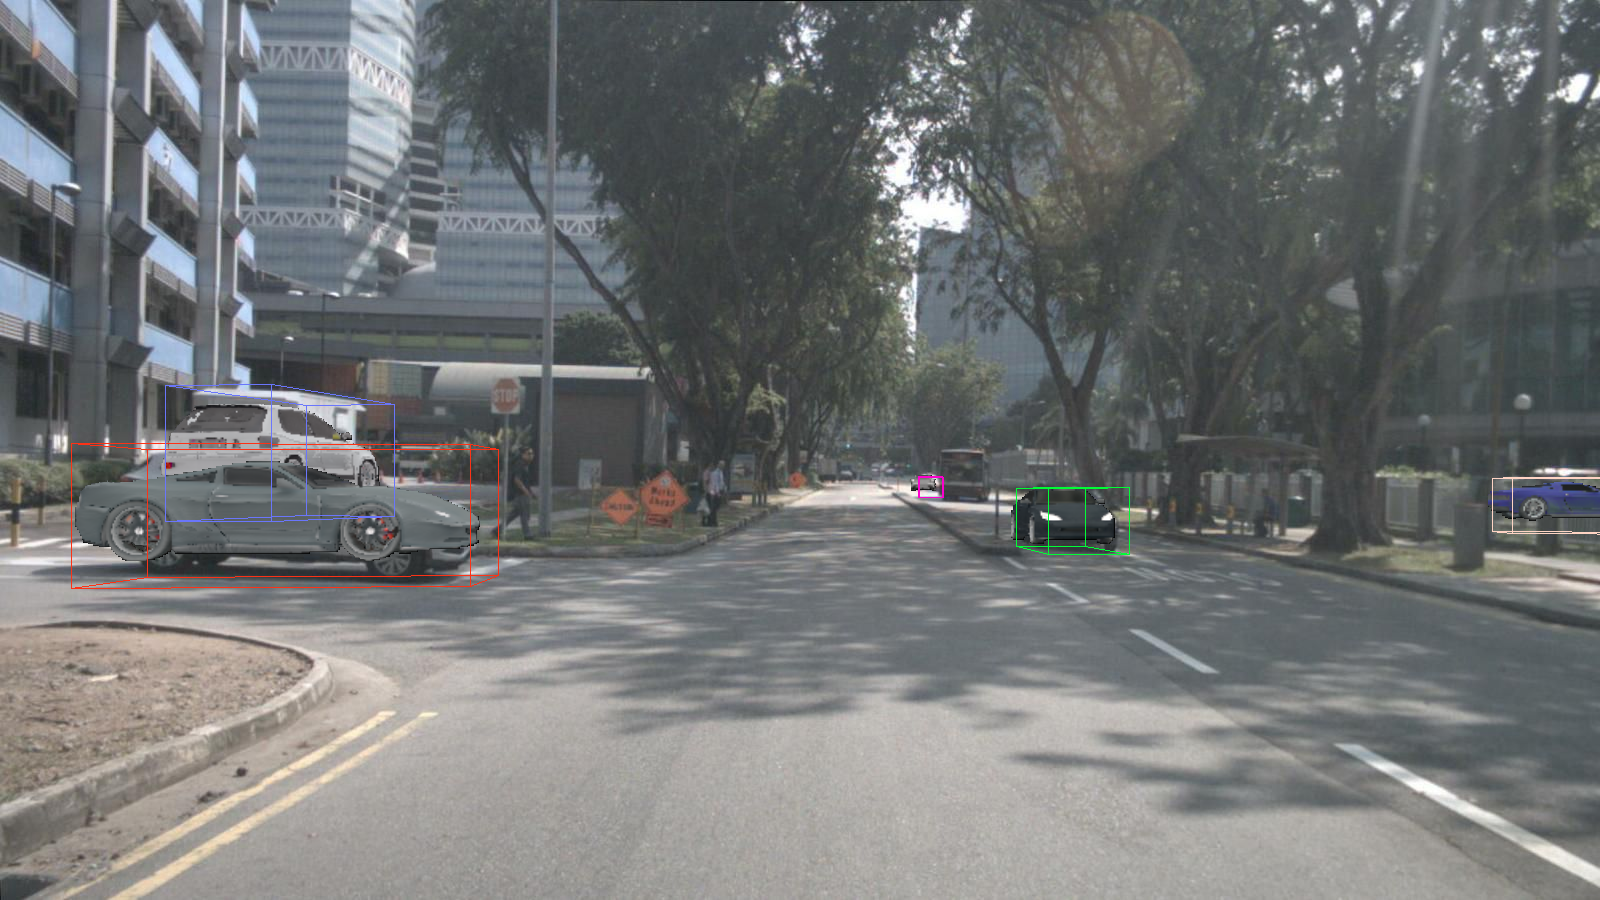
\includegraphics[width=.19\columnwidth, trim={0cm 0cm 0cm 0cm},clip]{fig/nuScenes_main/scene6/35_29_bbox.png}}&
% 		\raisebox{-0.5\height}{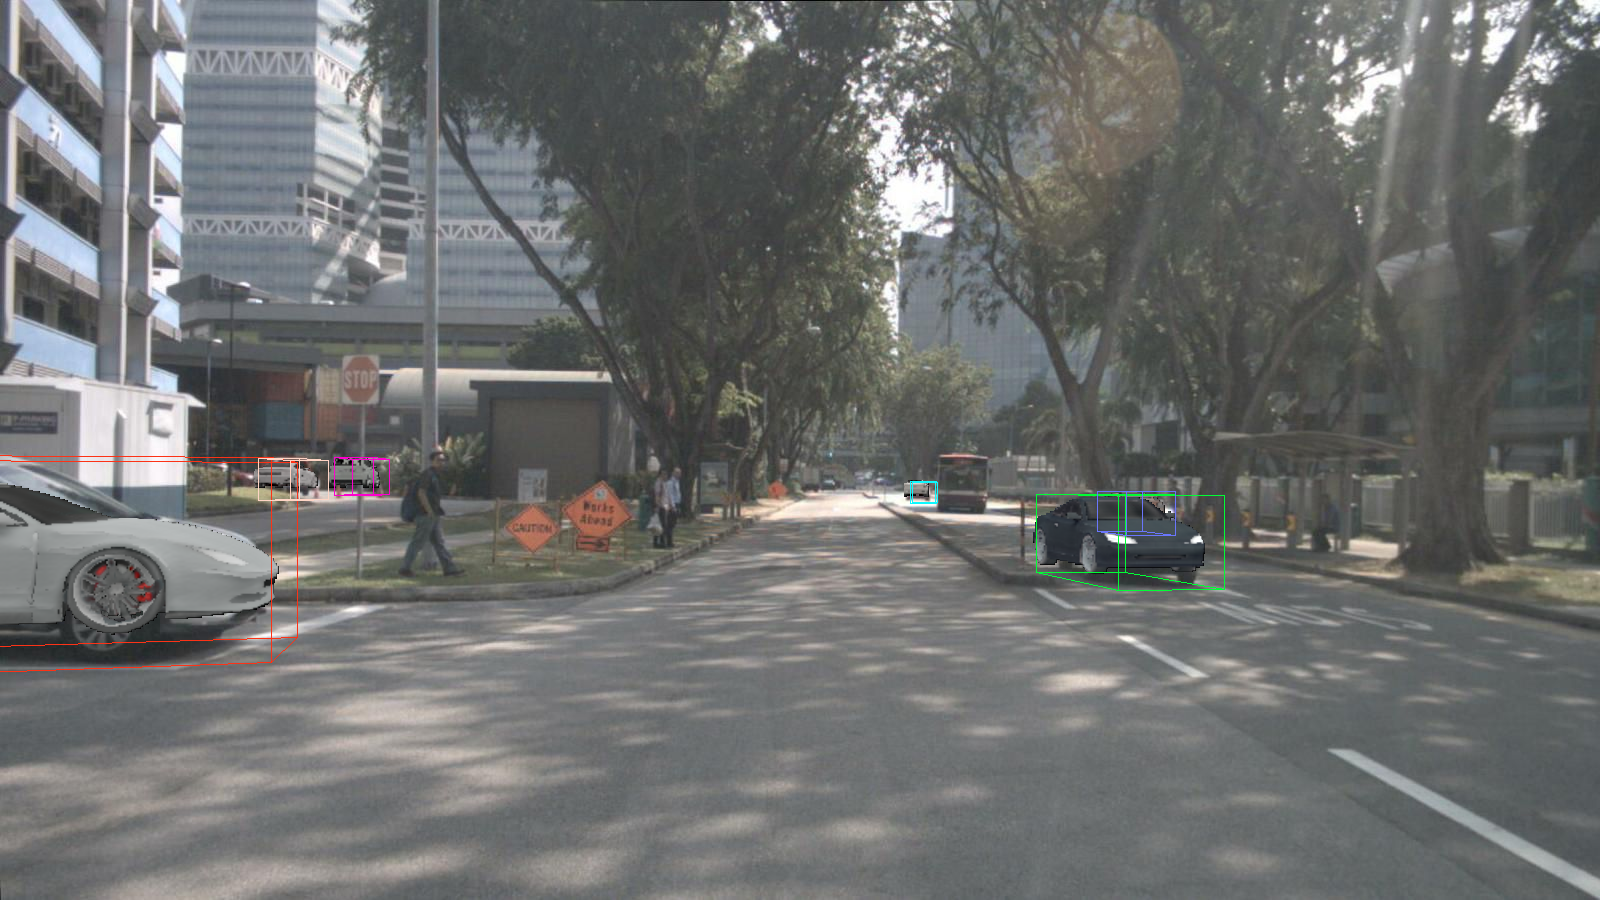
\includegraphics[width=.19\columnwidth, trim={0cm 0cm 0cm 0cm},clip]{fig/nuScenes_main/scene6/35_30_bbox.png}}&
% 		\raisebox{-0.5\height}{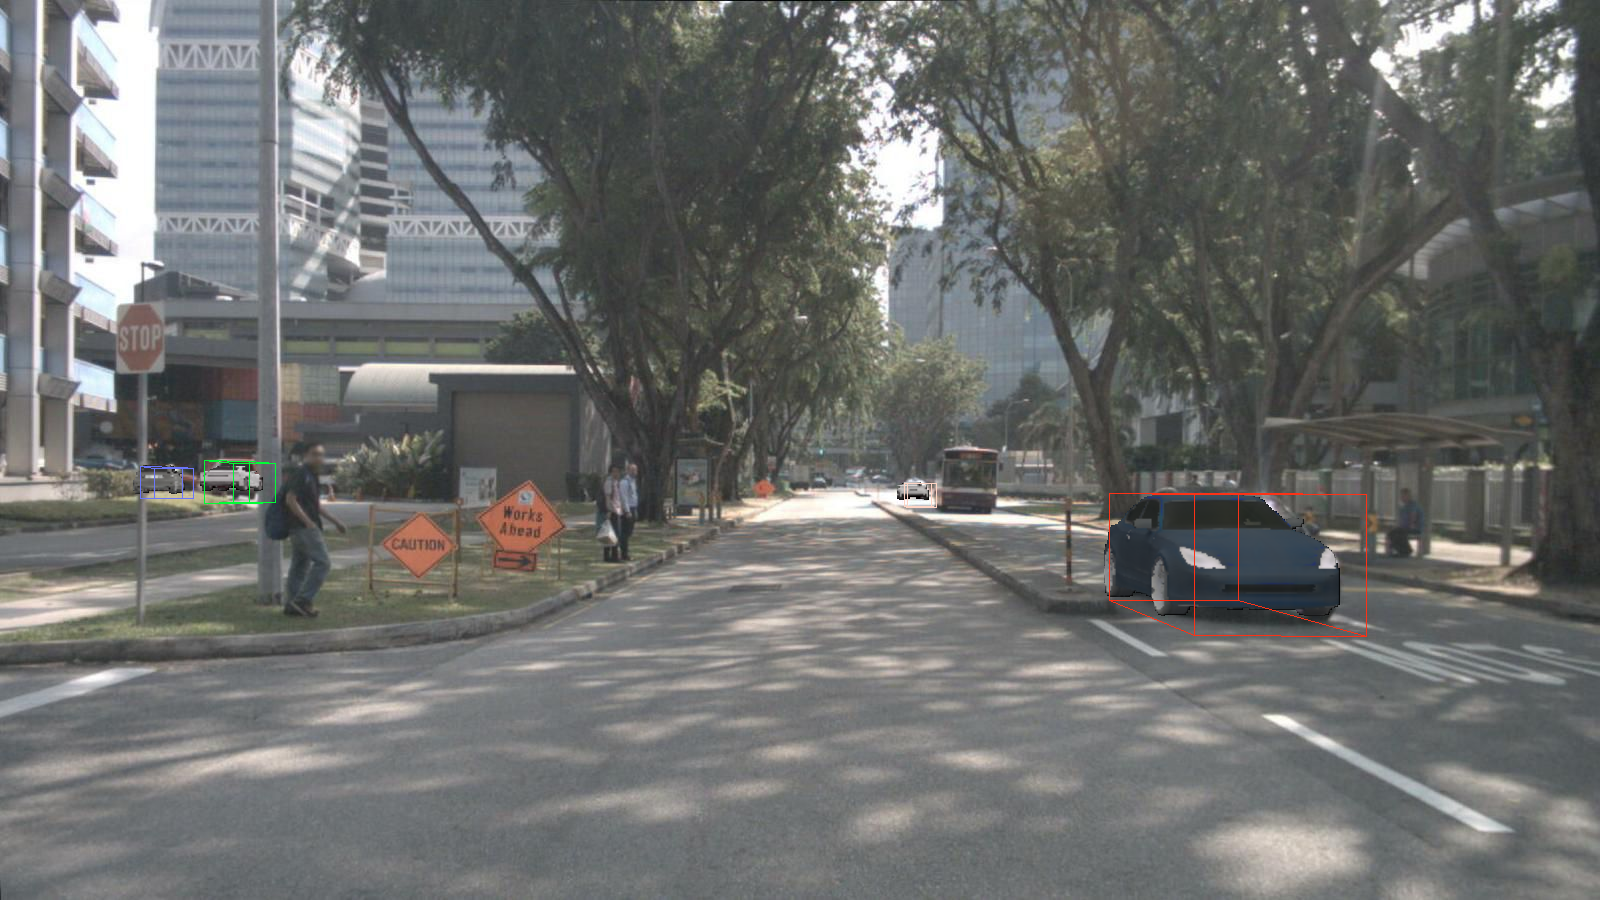
\includegraphics[width=.19\columnwidth, trim={0cm 0cm 0cm 0cm},clip]{fig/nuScenes_main/scene6/35_31_bbox.png}}\\[0.7cm]
  
%             \rotatebox[origin=c]{90}{{\footnotesize	Parking lot}}&
%   		\raisebox{-0.5\height}{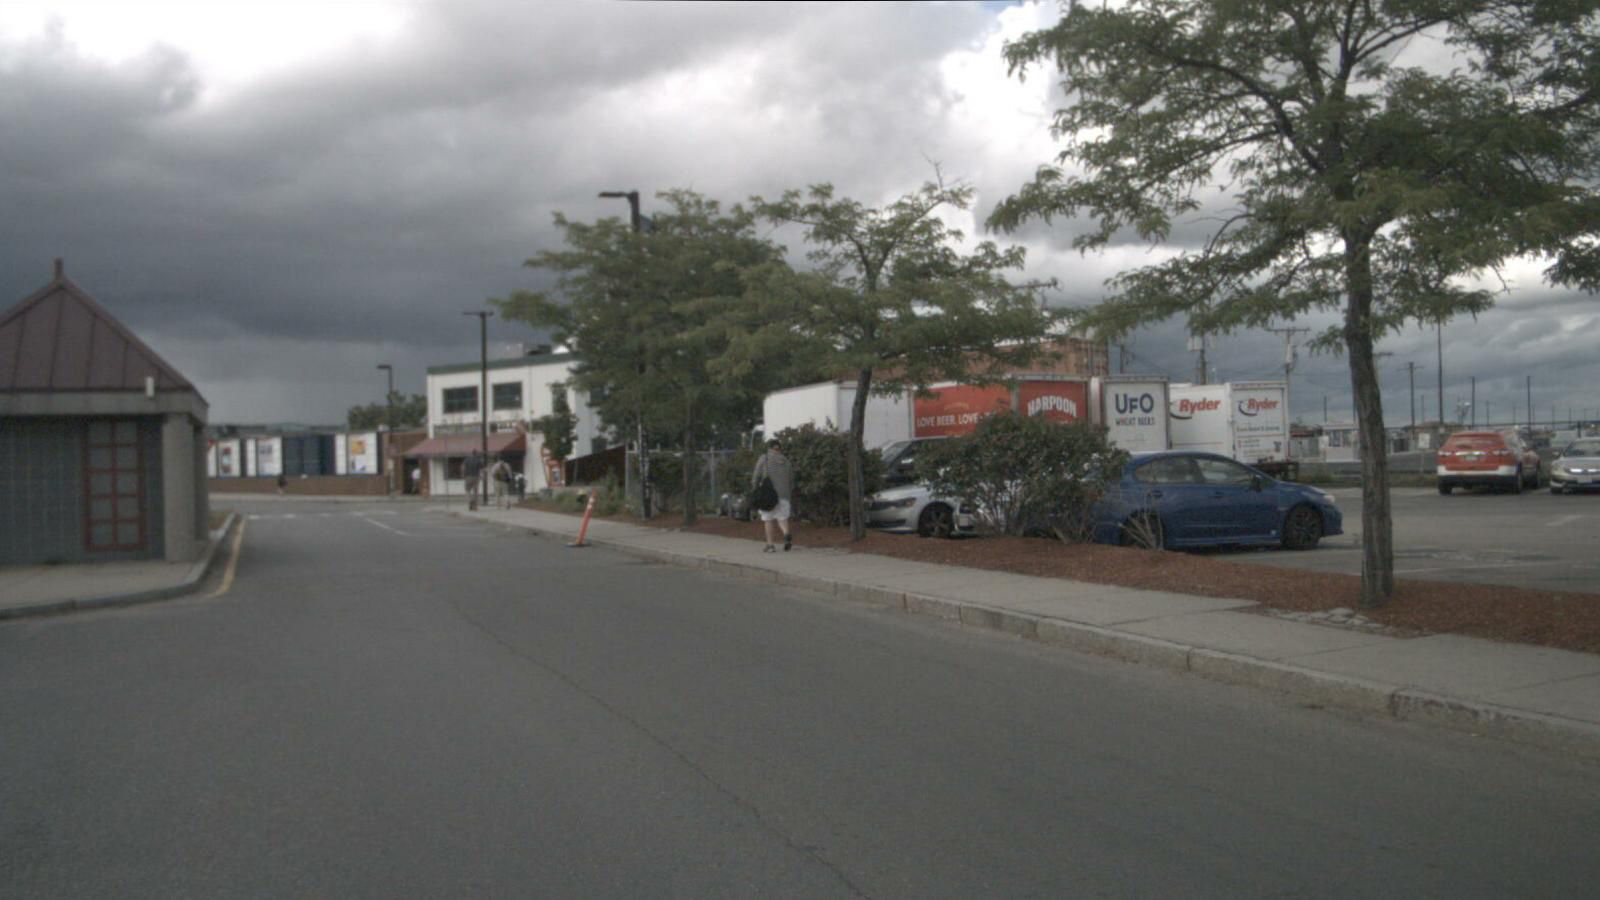
\includegraphics[width=.19\columnwidth, trim={0cm 0cm 0cm 0cm},clip]{fig/nuScenes_main/scene7/gt_2.png}}&
% 		\raisebox{-0.5\height}{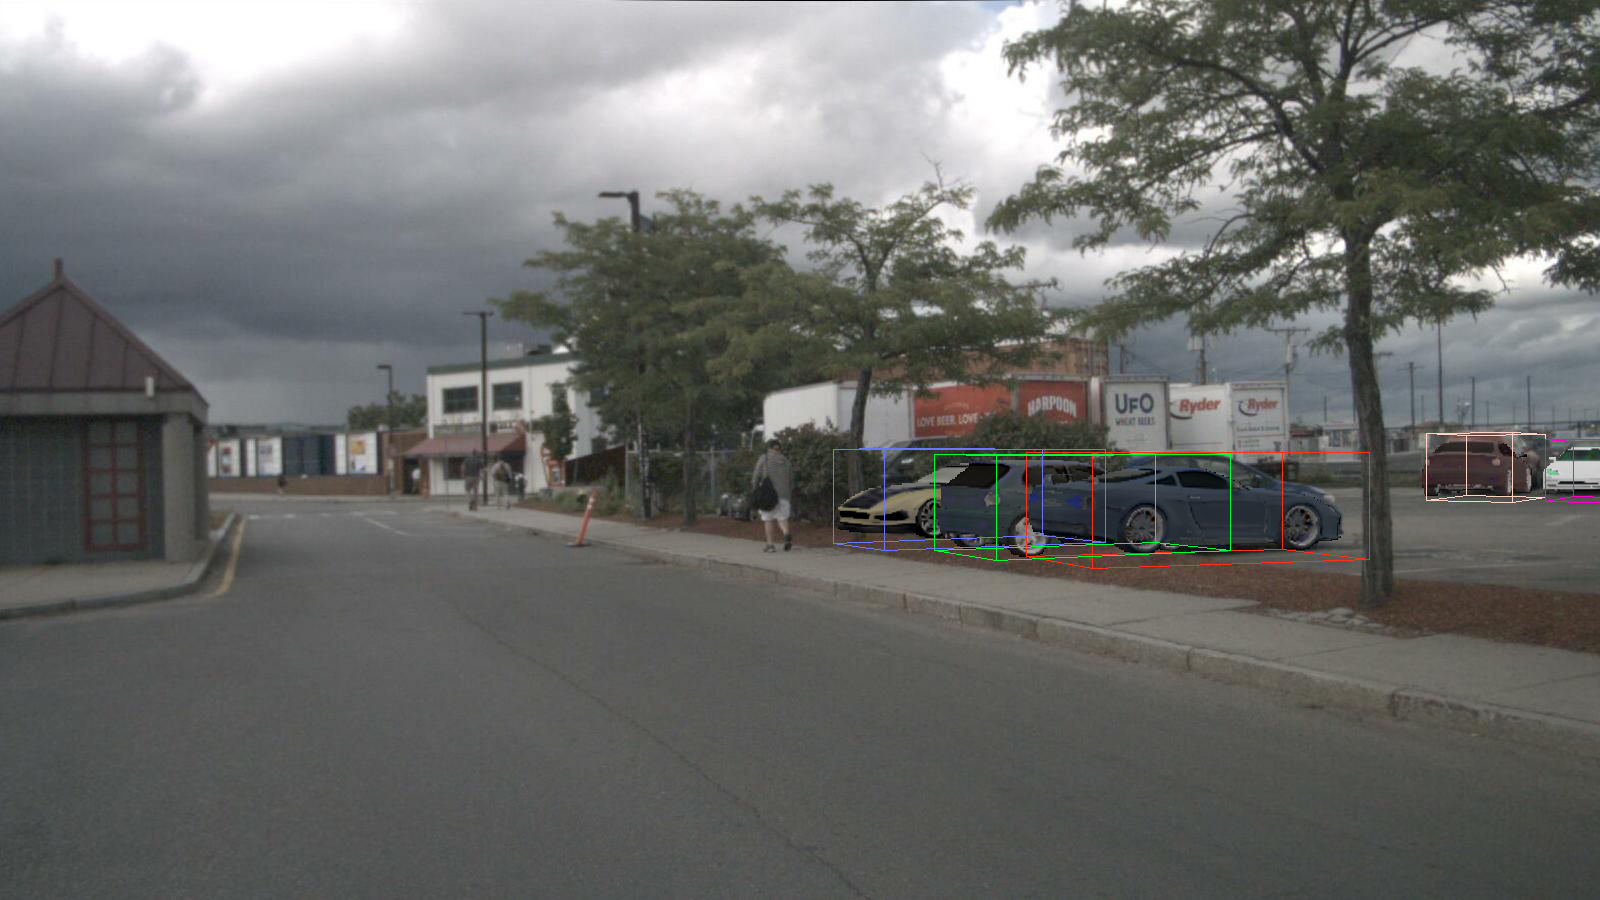
\includegraphics[width=.19\columnwidth, trim={0cm 0cm 0cm 0cm},clip]{fig/nuScenes_main/scene7/bbox_0.png}}&
% 		\raisebox{-0.5\height}{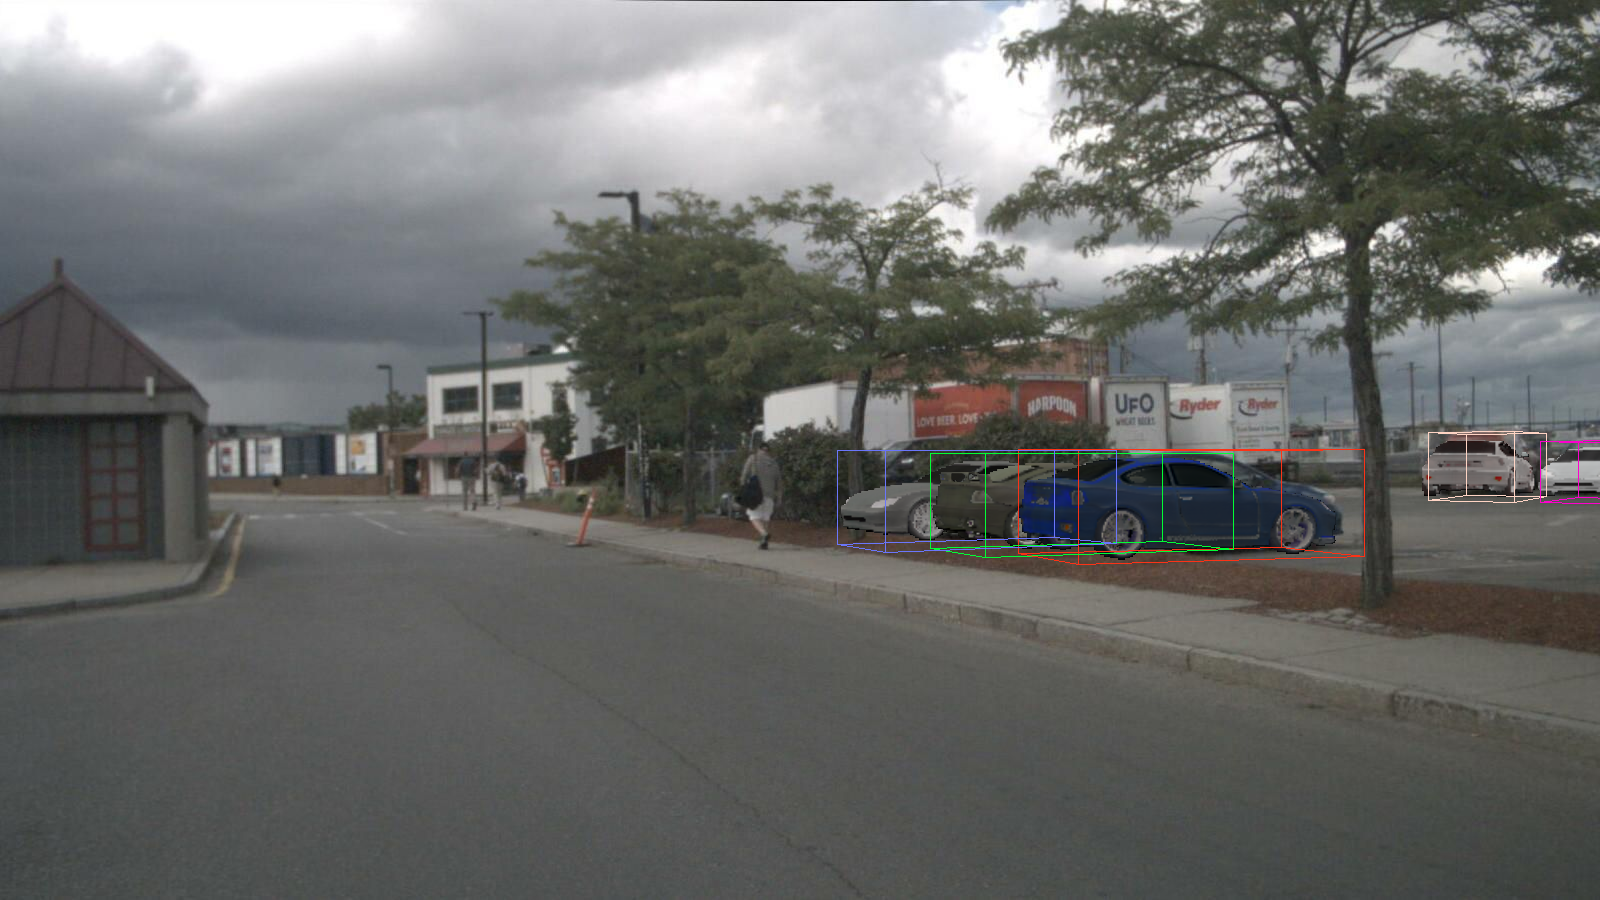
\includegraphics[width=.19\columnwidth, trim={0cm 0cm 0cm 0cm},clip]{fig/nuScenes_main/scene7/bbox_1.png}}&
% 		\raisebox{-0.5\height}{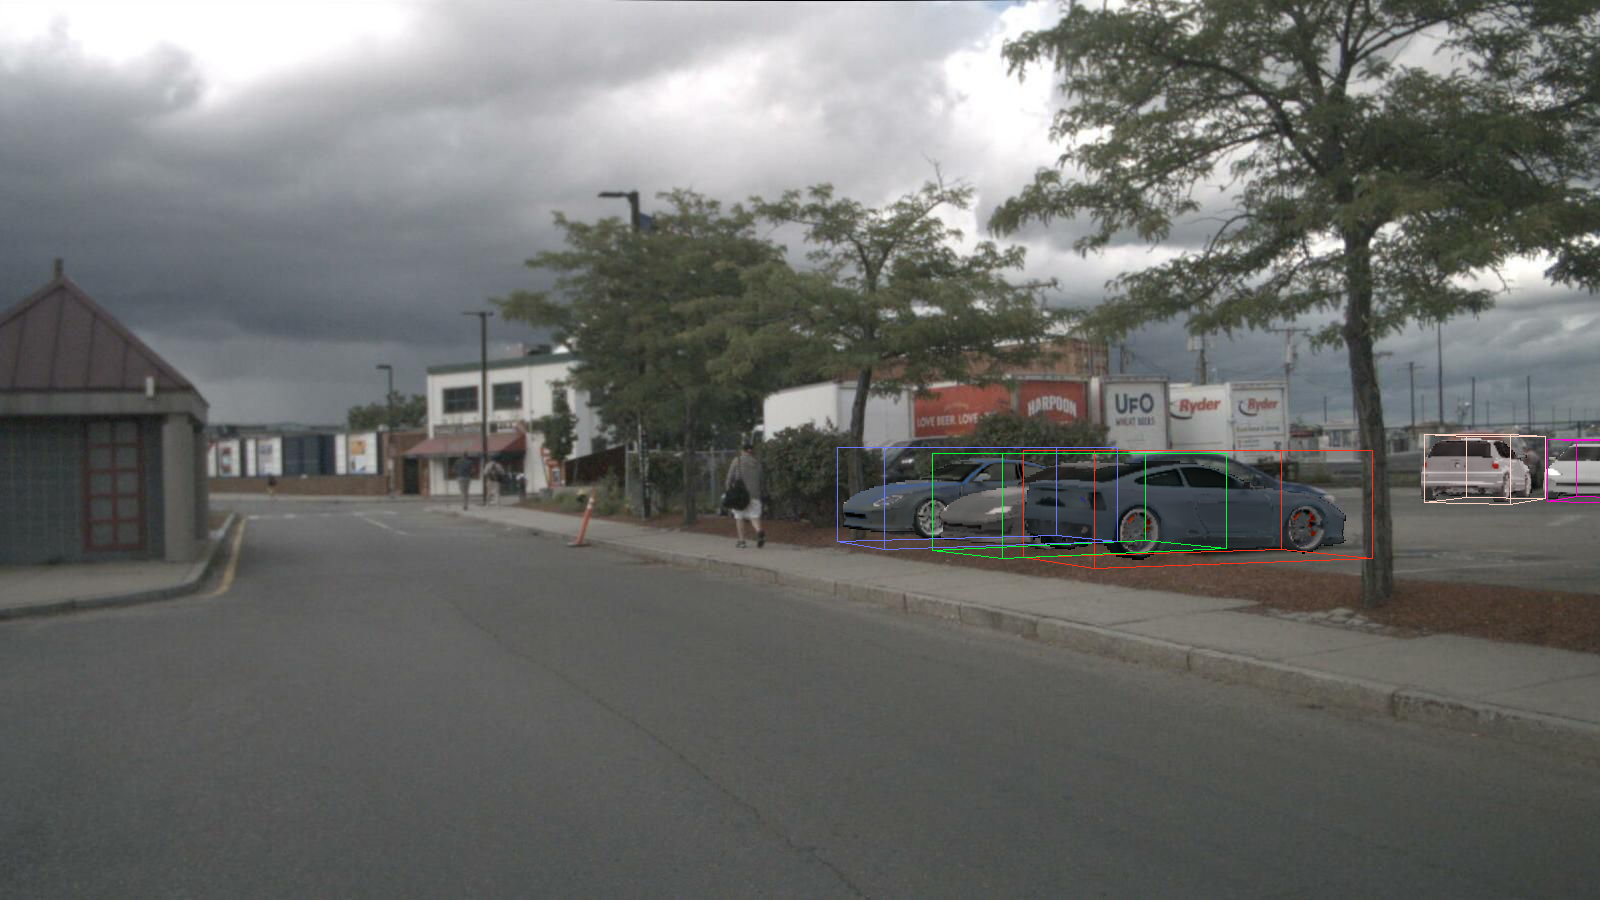
\includegraphics[width=.19\columnwidth, trim={0cm 0cm 0cm 0cm},clip]{fig/nuScenes_main/scene7/bbox_3.png}}&
% 		\raisebox{-0.5\height}{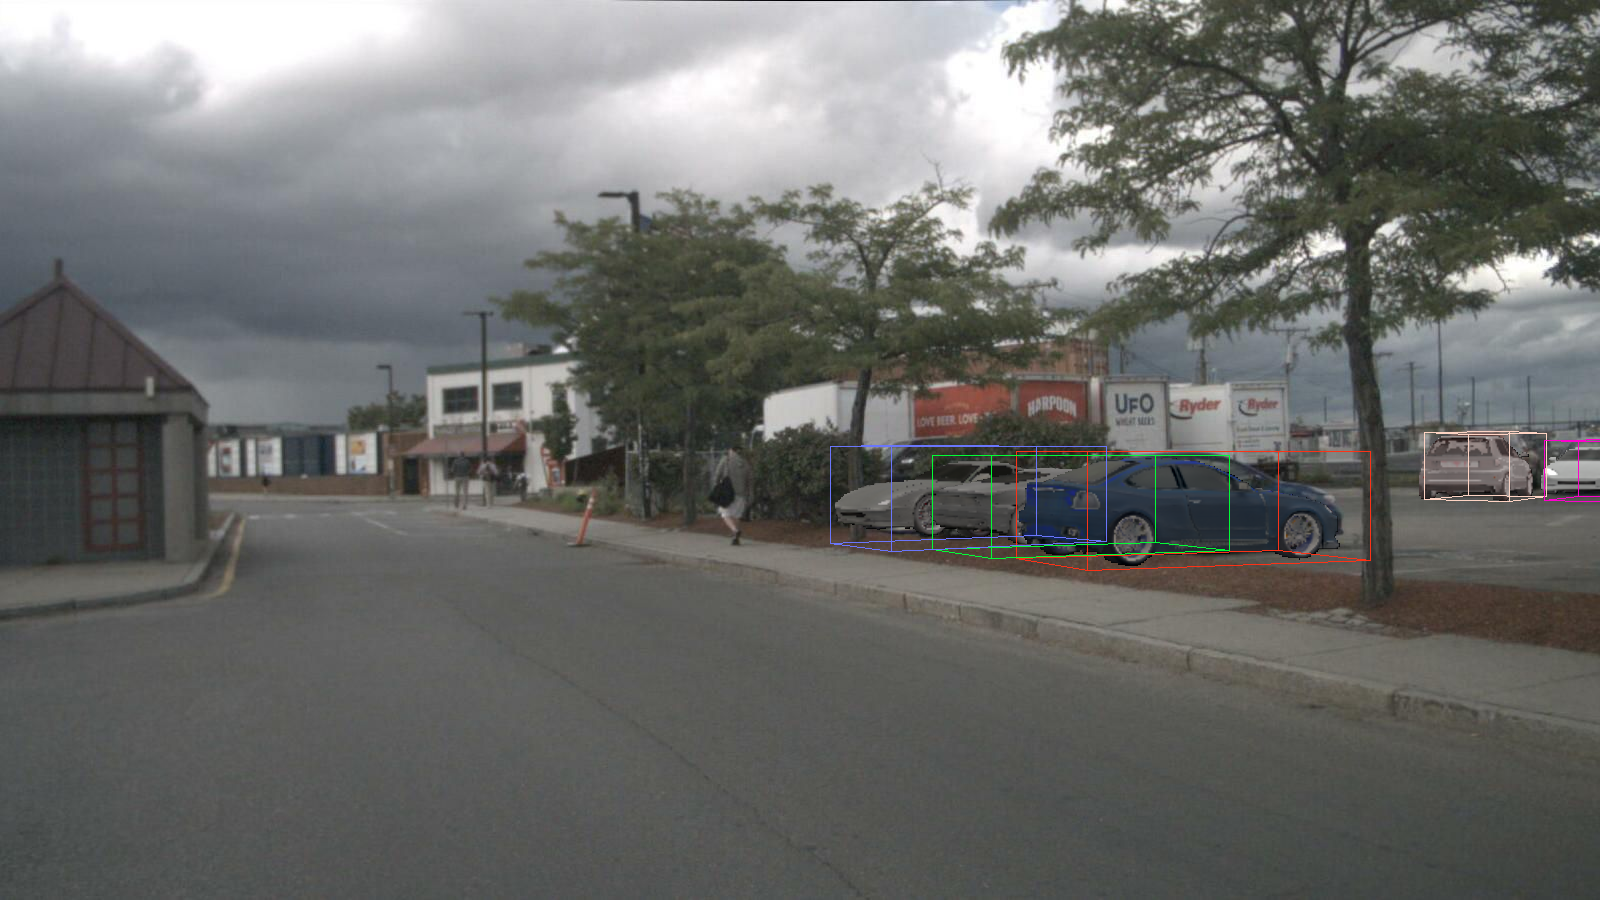
\includegraphics[width=.19\columnwidth, trim={0cm 0cm 0cm 0cm},clip]{fig/nuScenes_main/scene7/bbox_33.png}}\\%[0.95cm]
		
% 	\end{tabular}
% }
% 	\vspace{-6pt}
% 	\caption{Tracking via Inverse Neural Rendering on nuScenes~\cite{caesar2020nuscenes}. From left to right, we show (i) observed images from diverse scenes at timestep $k=0$; (ii) an overlay of the optimized generated object and its 3D bounding boxes at timestep $k=0, 1, 2 \text{ and } 3$. The color of the bounding boxes for each object corresponds to the predicted tracklet ID. We see that even in such diverse scenarios, our method does not lose any tracks and performs robustly across all scenarios, although the dataset is unseen.}
% 	\label{fig:nuScenes_results}
%  	\vspace{-12pt}
% \end{figure*}

\begin{figure*}[t!]
	% \vspace{-20pt}
	\centering
	\resizebox{1.\linewidth}{!}{
	\renewcommand{\arraystretch}{0.5}
	\begin{tabular}{@{}c@{\hskip 0.05cm}c@{\hskip 0.05cm}c@{\hskip 0.05cm}c@{\hskip 0.05cm}c@{\hskip 0.05cm}c@{}}
		\centering
            &
		{\small Input $t_0$}&
		{\small Tracked $t_0$}&
		{\small Tracked $t_1$}&
		{\small Tracked $t_2$}&
		{\small Tracked $t_3$}\\

            \rotatebox[origin=c]{90}{{\footnotesize	  Suburban}}&
		 \raisebox{-0.5\height}{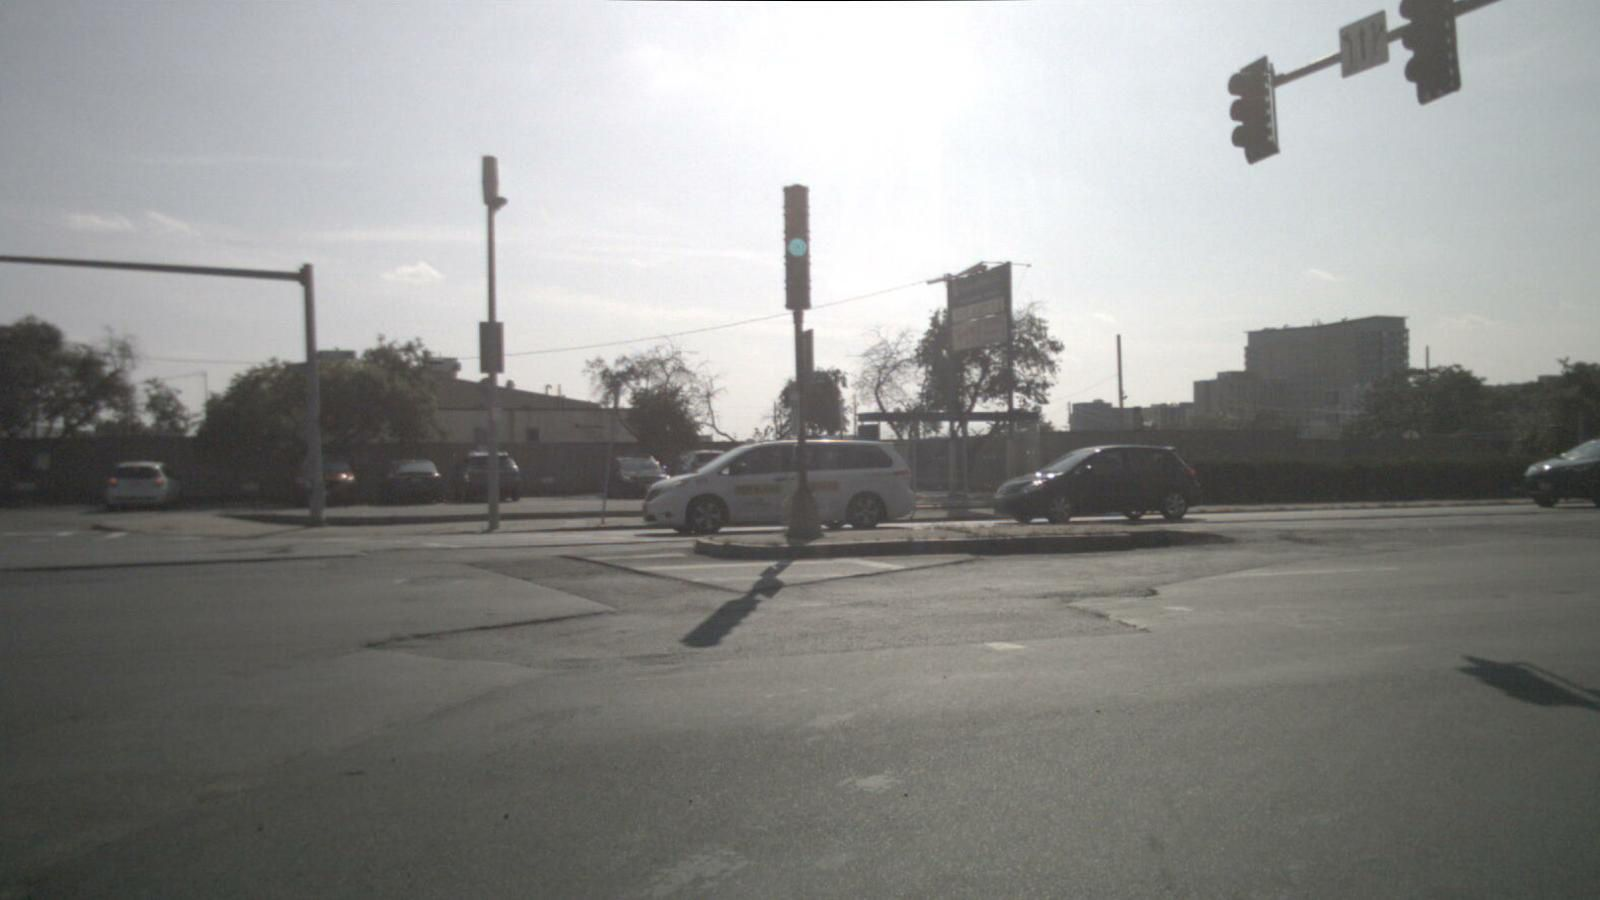
\includegraphics[width=.32\columnwidth, trim={0cm 0cm 0cm 0cm},clip]{fig/nuScenes_main/scene2/0484_2_gt.png}}&
		 \raisebox{-0.5\height}{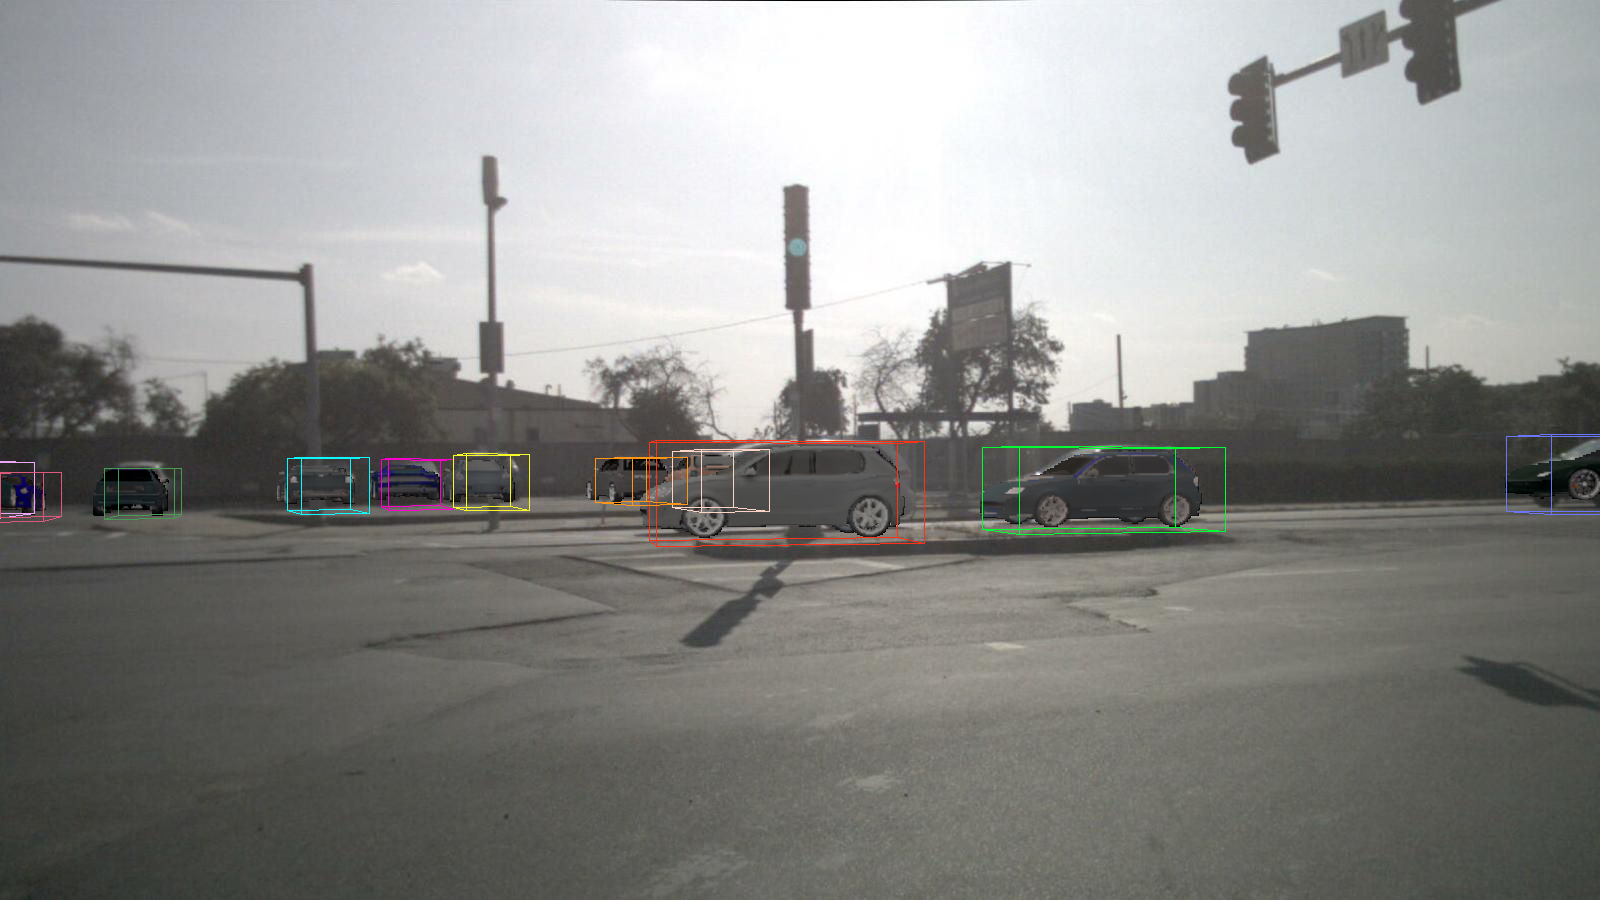
\includegraphics[width=.32\columnwidth, trim={0cm 0cm 0cm 0cm},clip]{fig/nuScenes_main/scene2/0484_2_bbox.png}}&
		 \raisebox{-0.5\height}{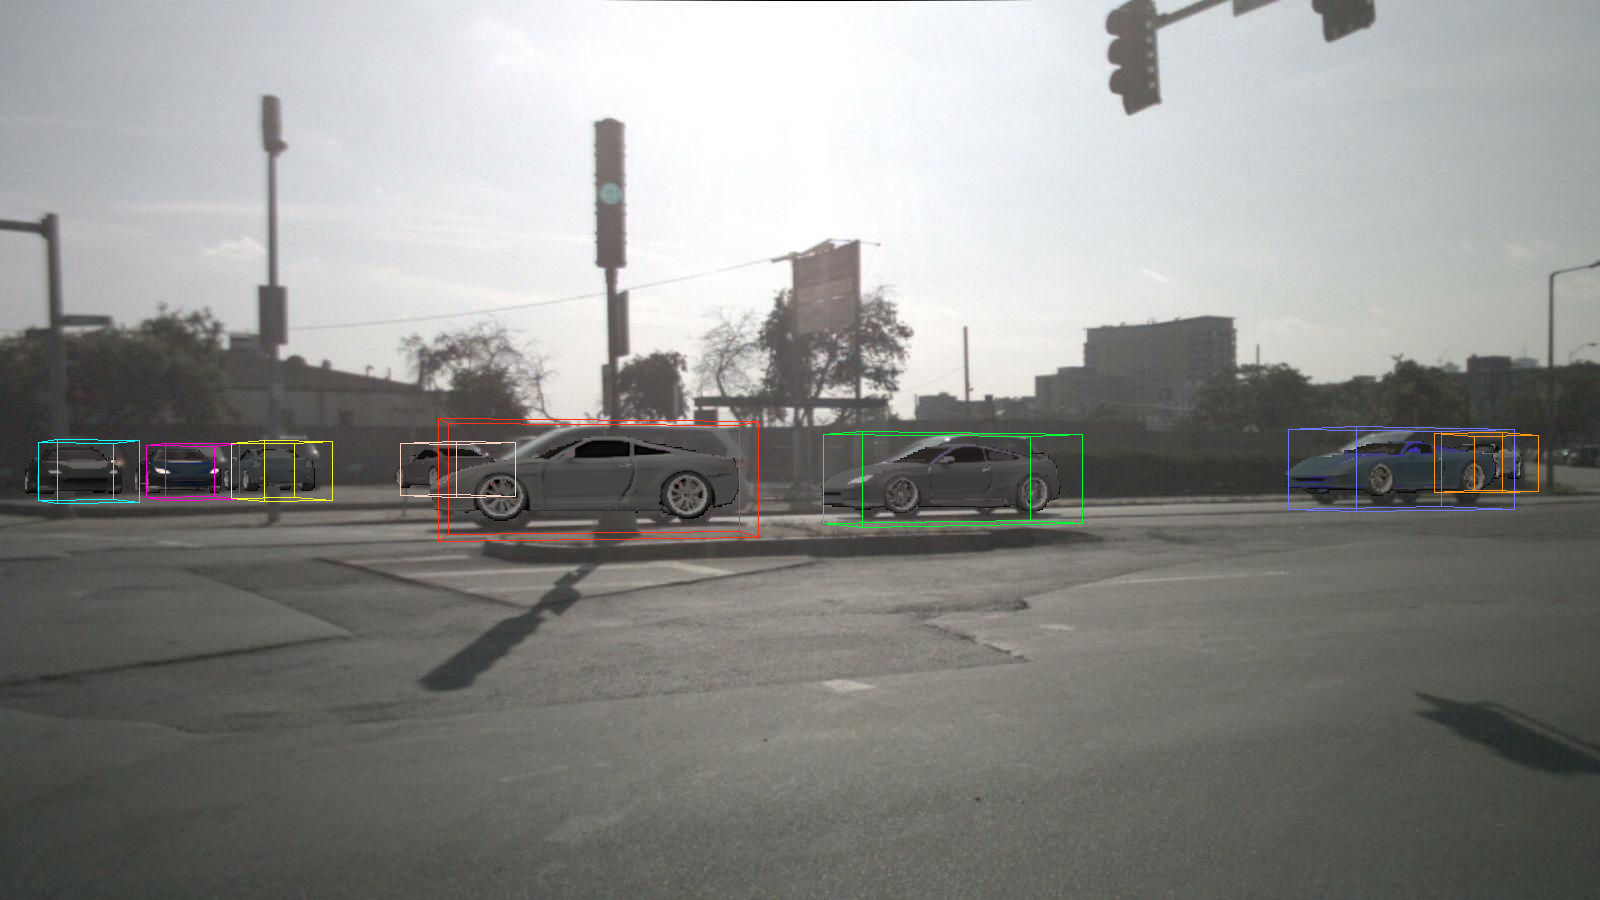
\includegraphics[width=.32\columnwidth, trim={0cm 0cm 0cm 0cm},clip]{fig/nuScenes_main/scene2/0484_3_bbox.png}}&
		 \raisebox{-0.5\height}{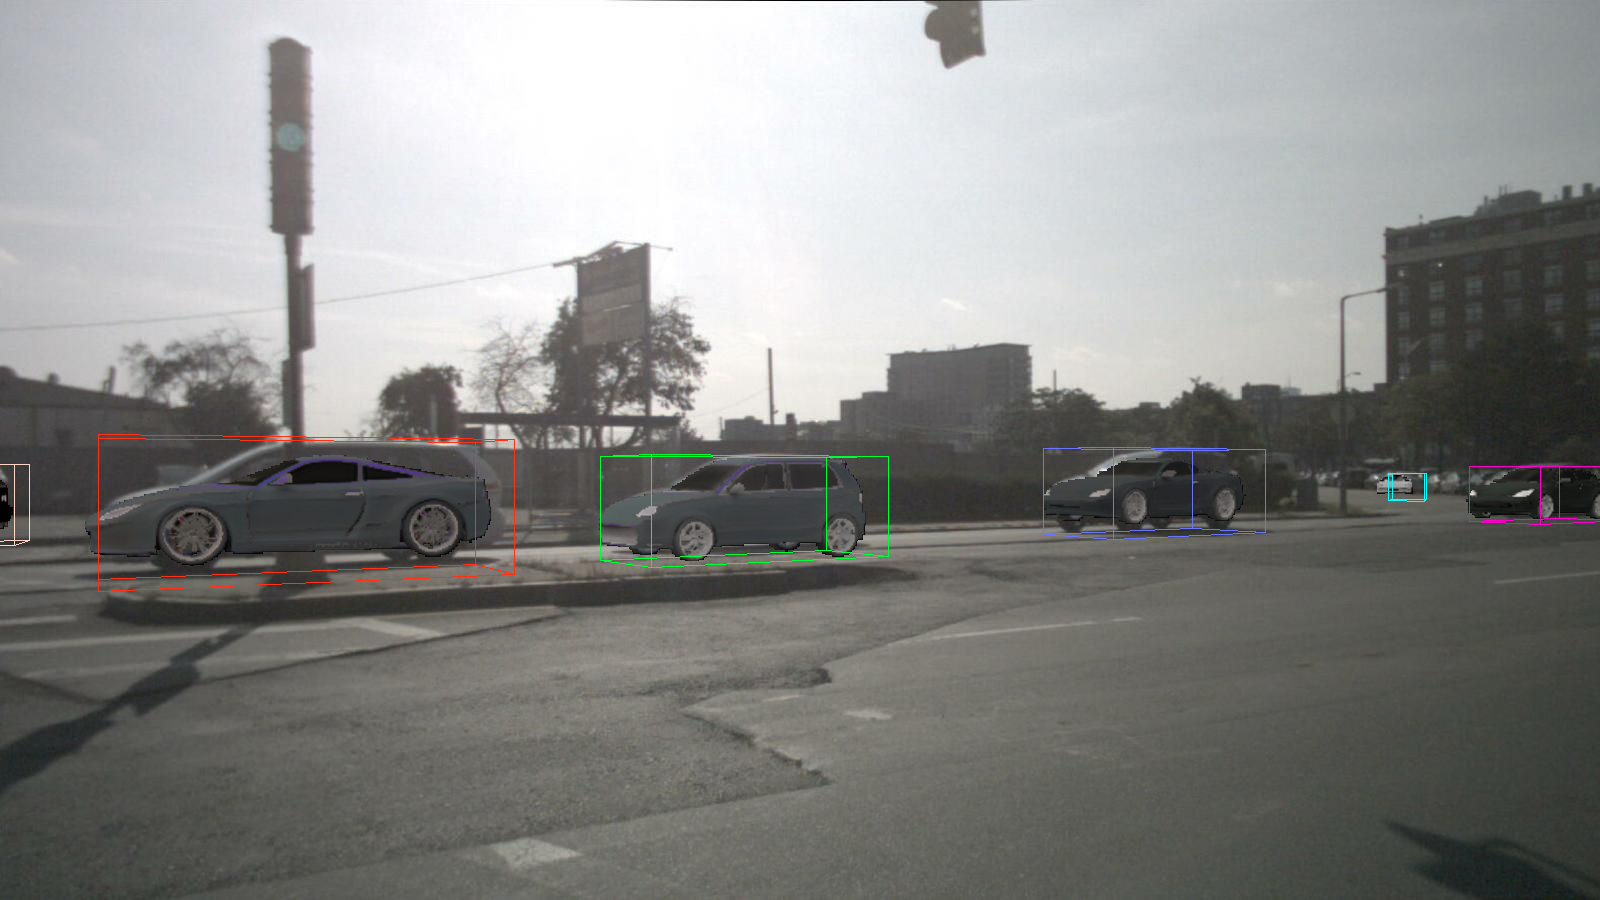
\includegraphics[width=.32\columnwidth, trim={0cm 0cm 0cm 0cm},clip]{fig/nuScenes_main/scene2/0484_4_bbox.png}}&
		 \raisebox{-0.5\height}{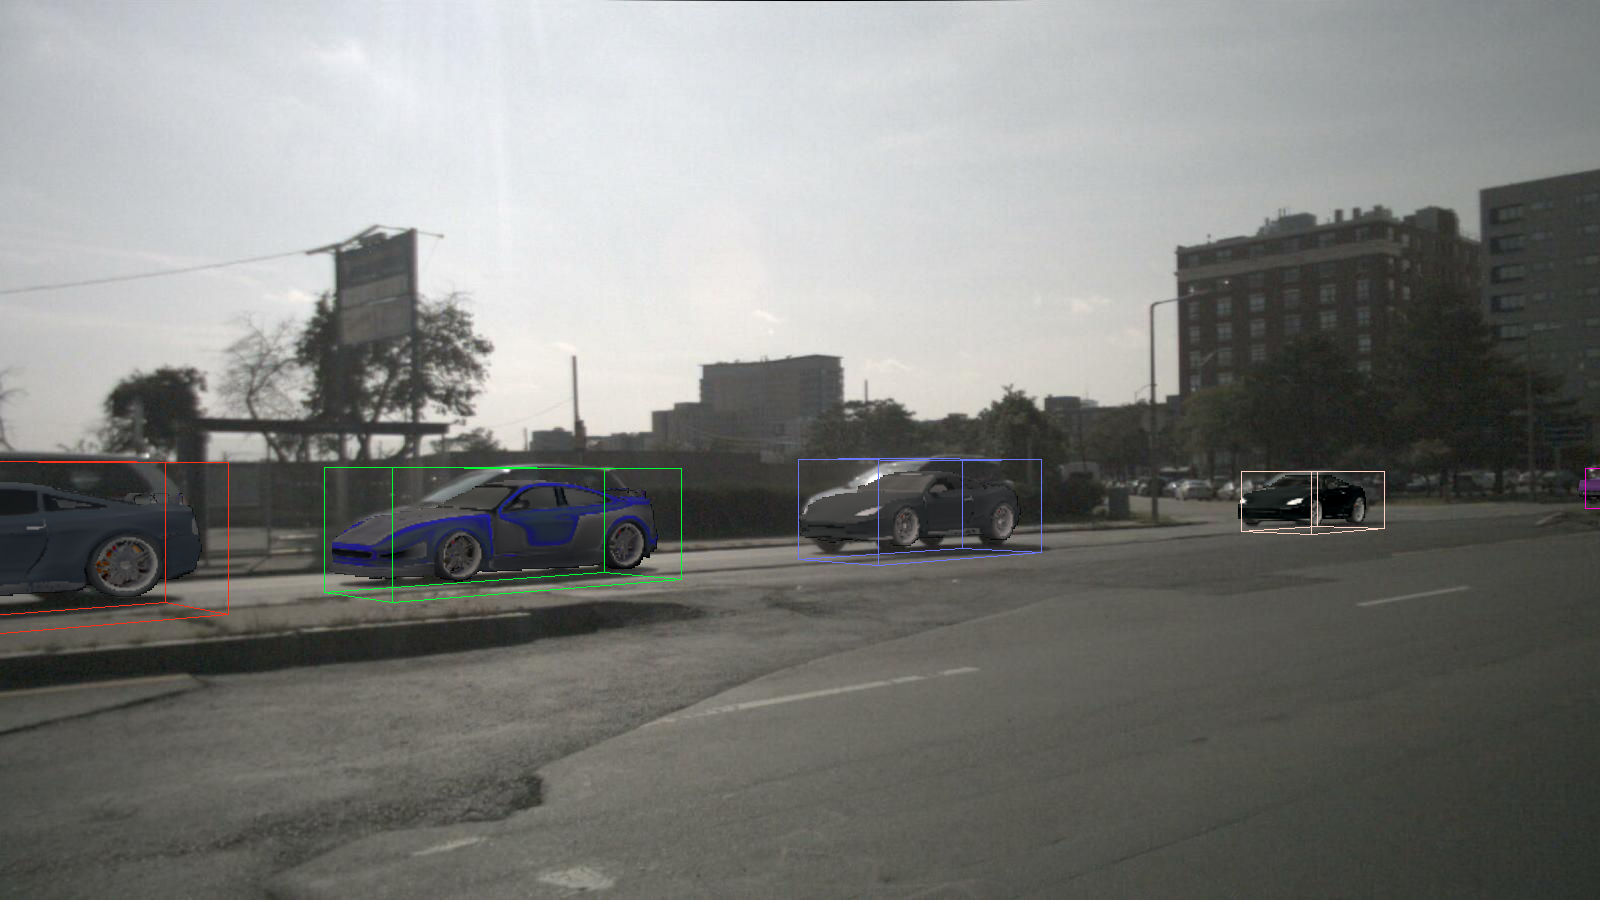
\includegraphics[width=.32\columnwidth, trim={0cm 0cm 0cm 0cm},clip]{fig/nuScenes_main/scene2/0484_5_bbox.png}}\\[1.1cm]
  
		\rotatebox[origin=c]{90}{{\footnotesize	 Dense Urban}}&
		\raisebox{-0.5\height}{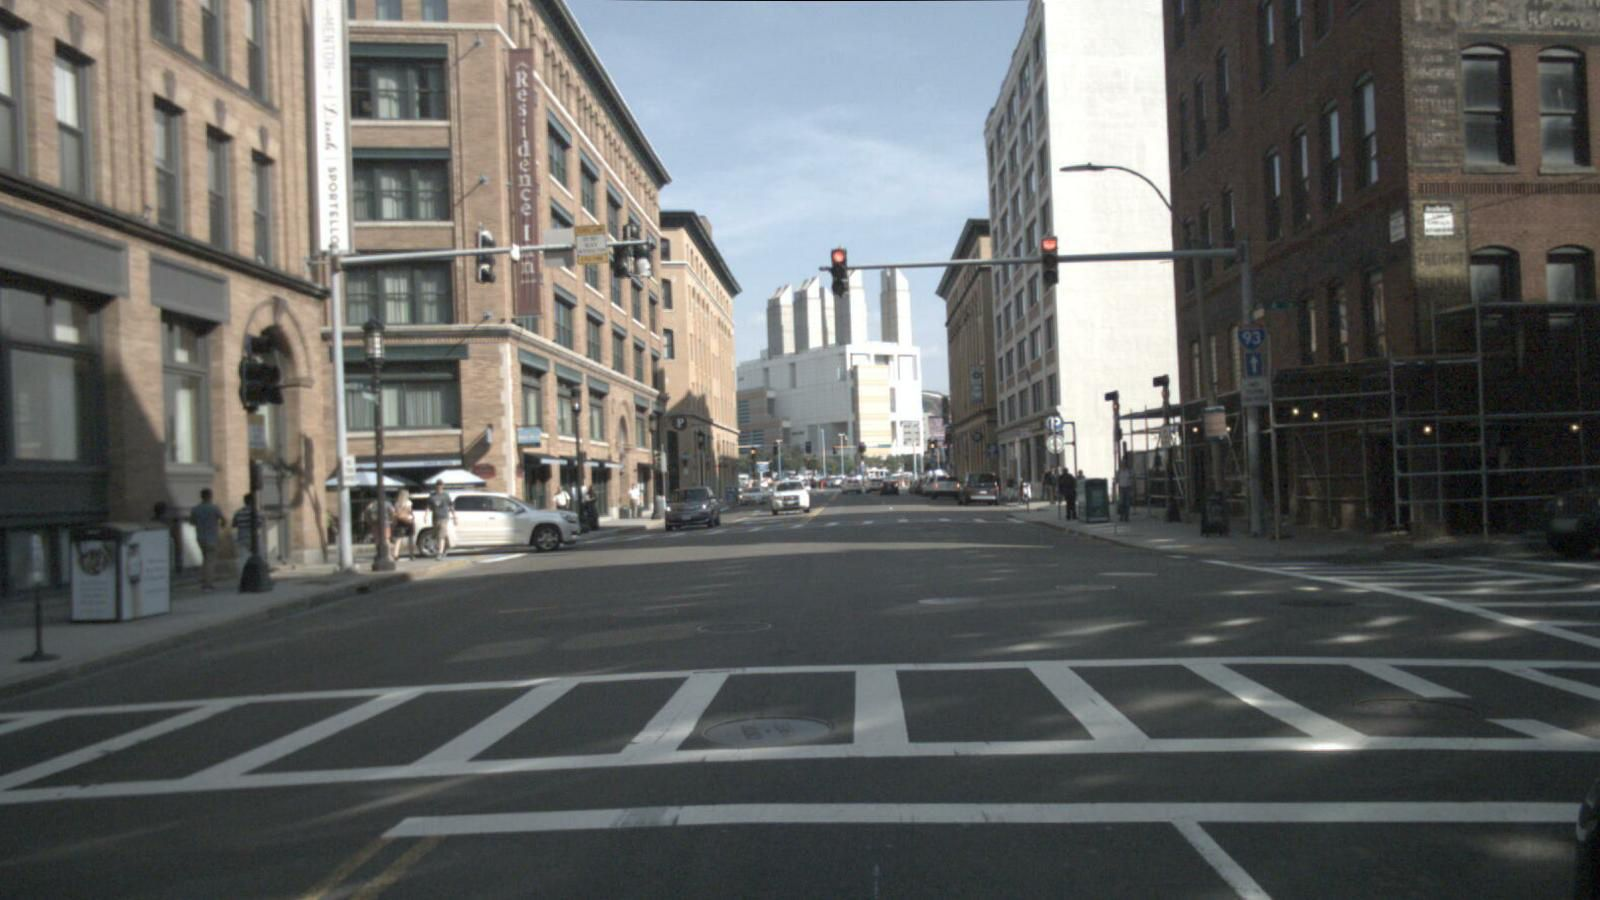
\includegraphics[width=.32\columnwidth, trim={0cm 0cm 0cm 0cm},clip]{fig/nuScenes_main/scene3/0496_30_gt.png}}&
		\raisebox{-0.5\height}{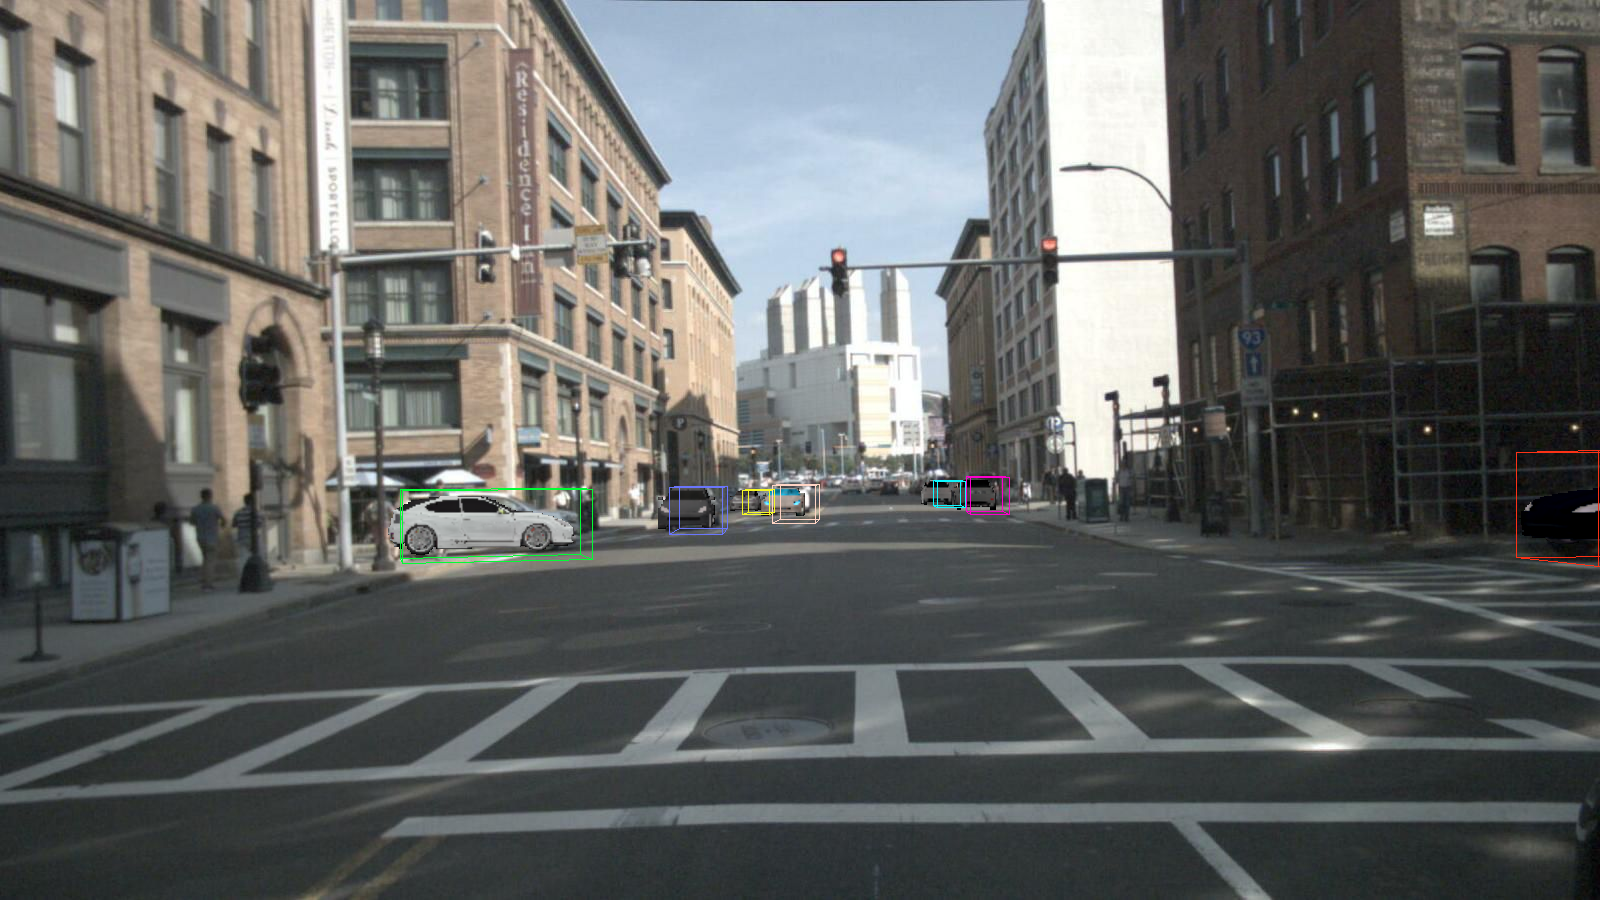
\includegraphics[width=.32\columnwidth, trim={0cm 0cm 0cm 0cm},clip]{fig/nuScenes_main/scene3/0496_30_bbox.png}} &
		\raisebox{-0.5\height}{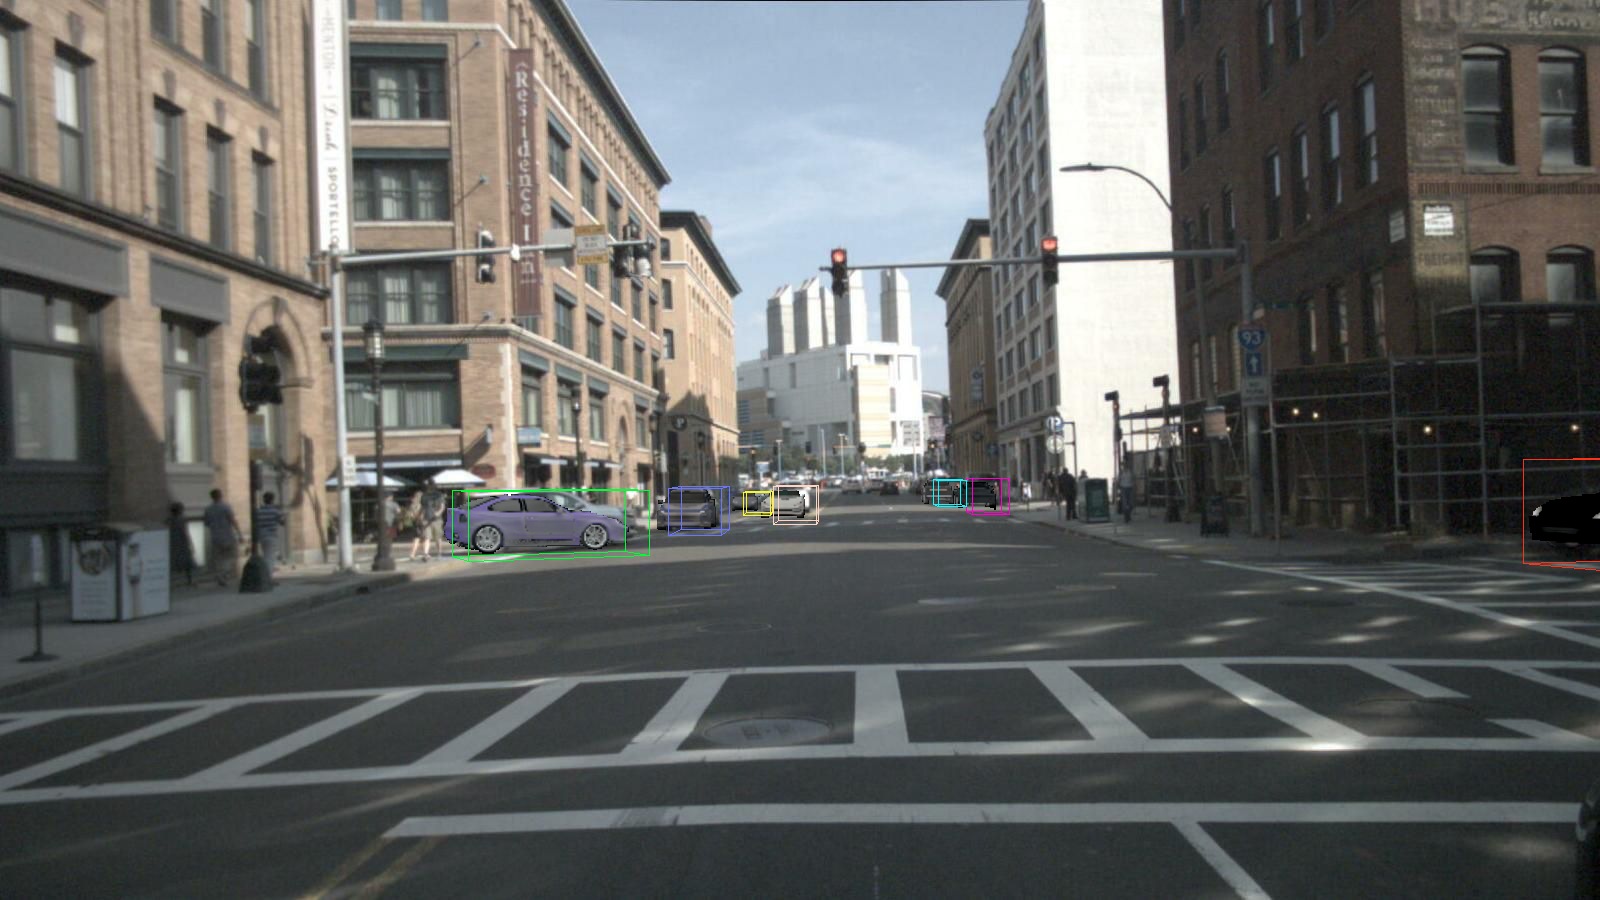
\includegraphics[width=.32\columnwidth, trim={0cm 0cm 0cm 0cm},clip]{fig/nuScenes_main/scene3/0496_31_bbox.png}}&
		\raisebox{-0.5\height}{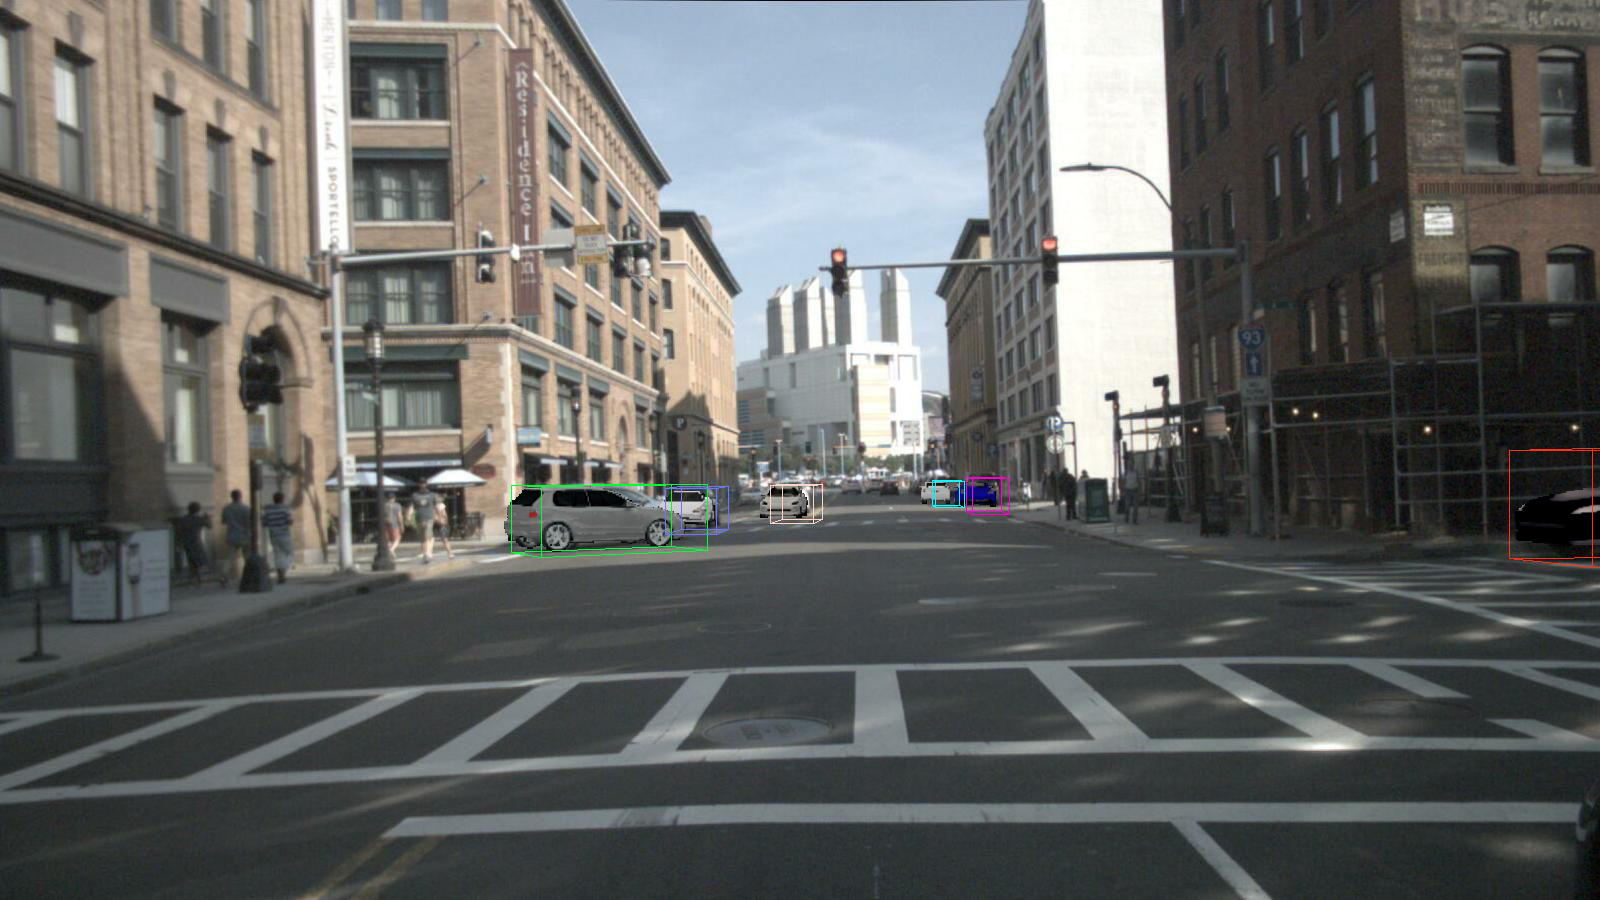
\includegraphics[width=.32\columnwidth, trim={0cm 0cm 0cm 0cm},clip]{fig/nuScenes_main/scene3/0496_32_bbox.png}}&
		\raisebox{-0.5\height}{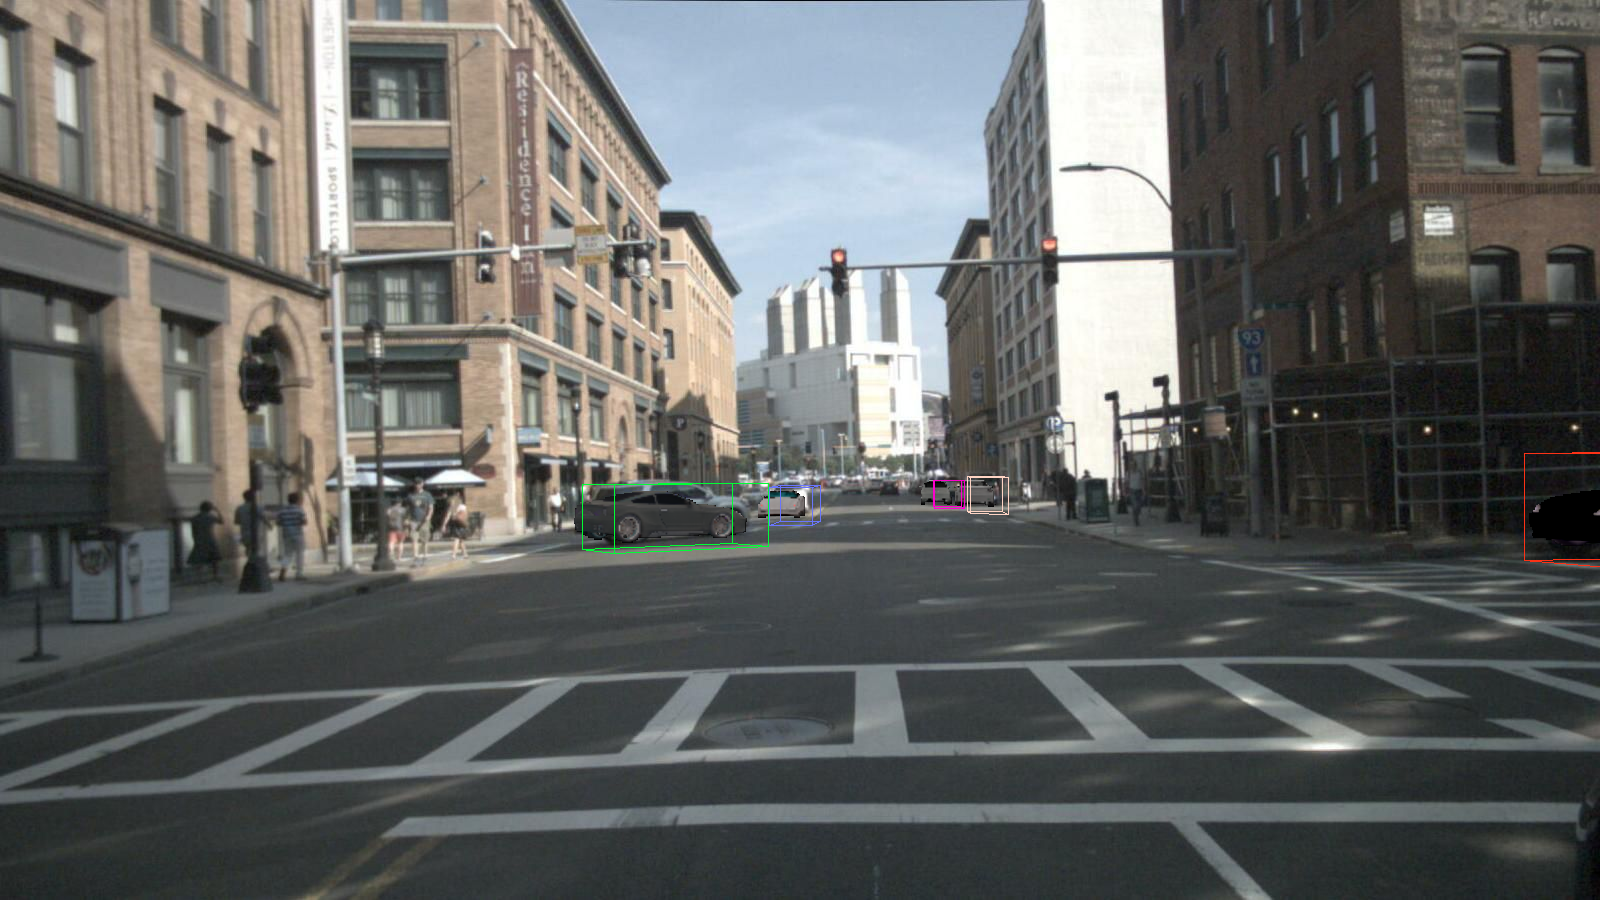
\includegraphics[width=.32\columnwidth, trim={0cm 0cm 0cm 0cm},clip]{fig/nuScenes_main/scene3/0496_33_bbox.png}}\\[1.1cm]
  
            \rotatebox[origin=c]{90}{{\footnotesize	 Clutter}}&
  		\raisebox{-0.5\height}{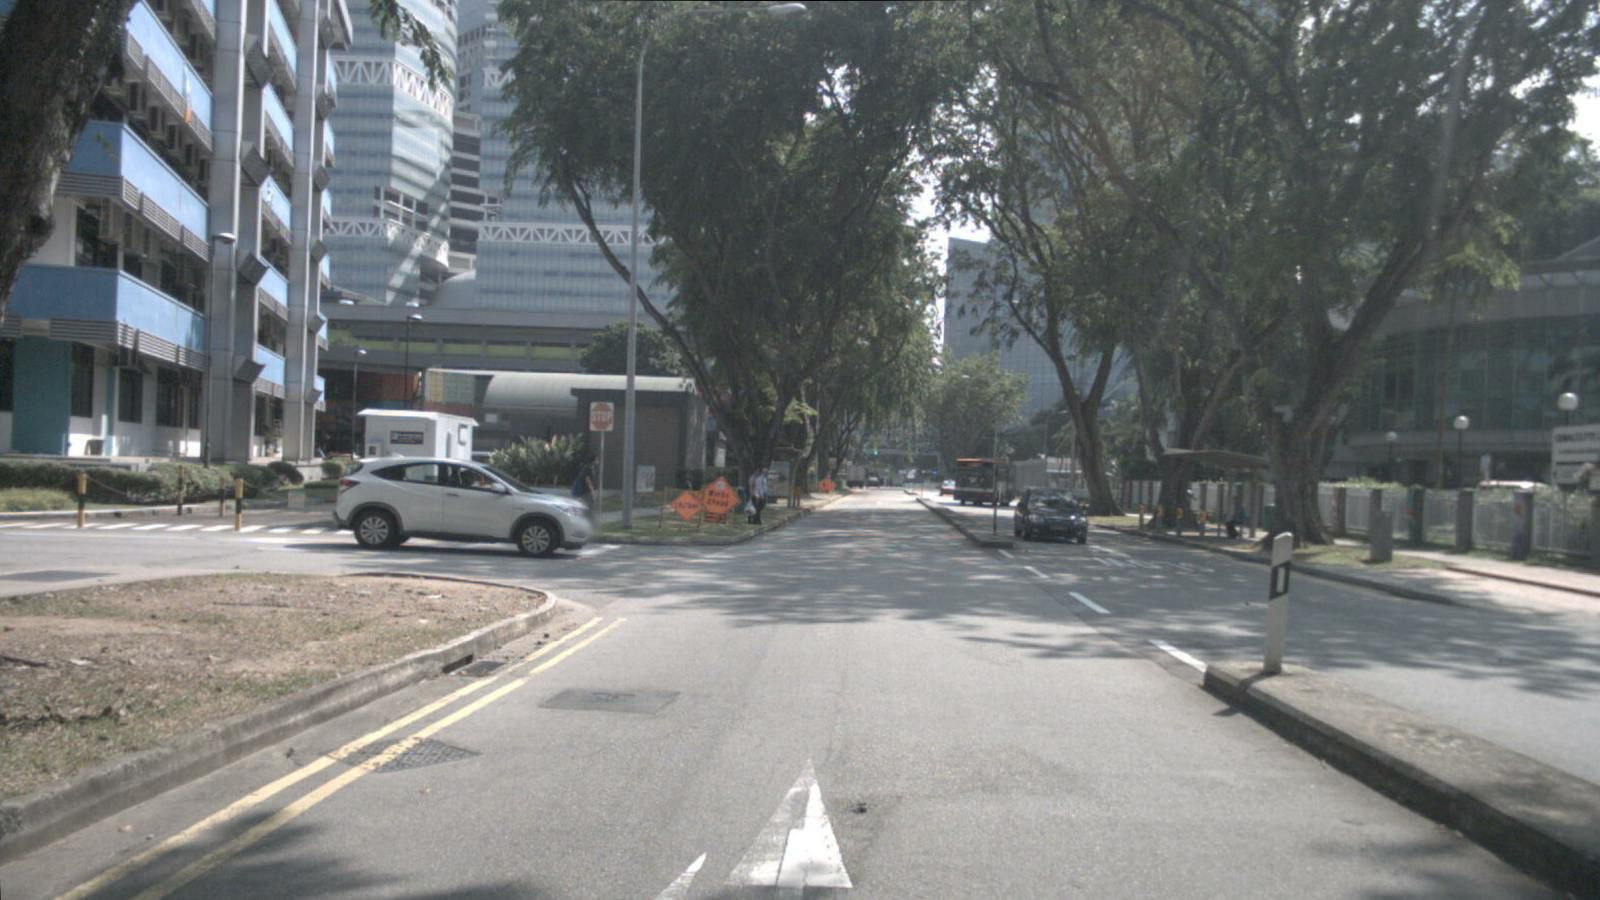
\includegraphics[width=.32\columnwidth, trim={0cm 0cm 0cm 0cm},clip]{fig/nuScenes_main/scene6/28_gt_img.png}}&
		\raisebox{-0.5\height}{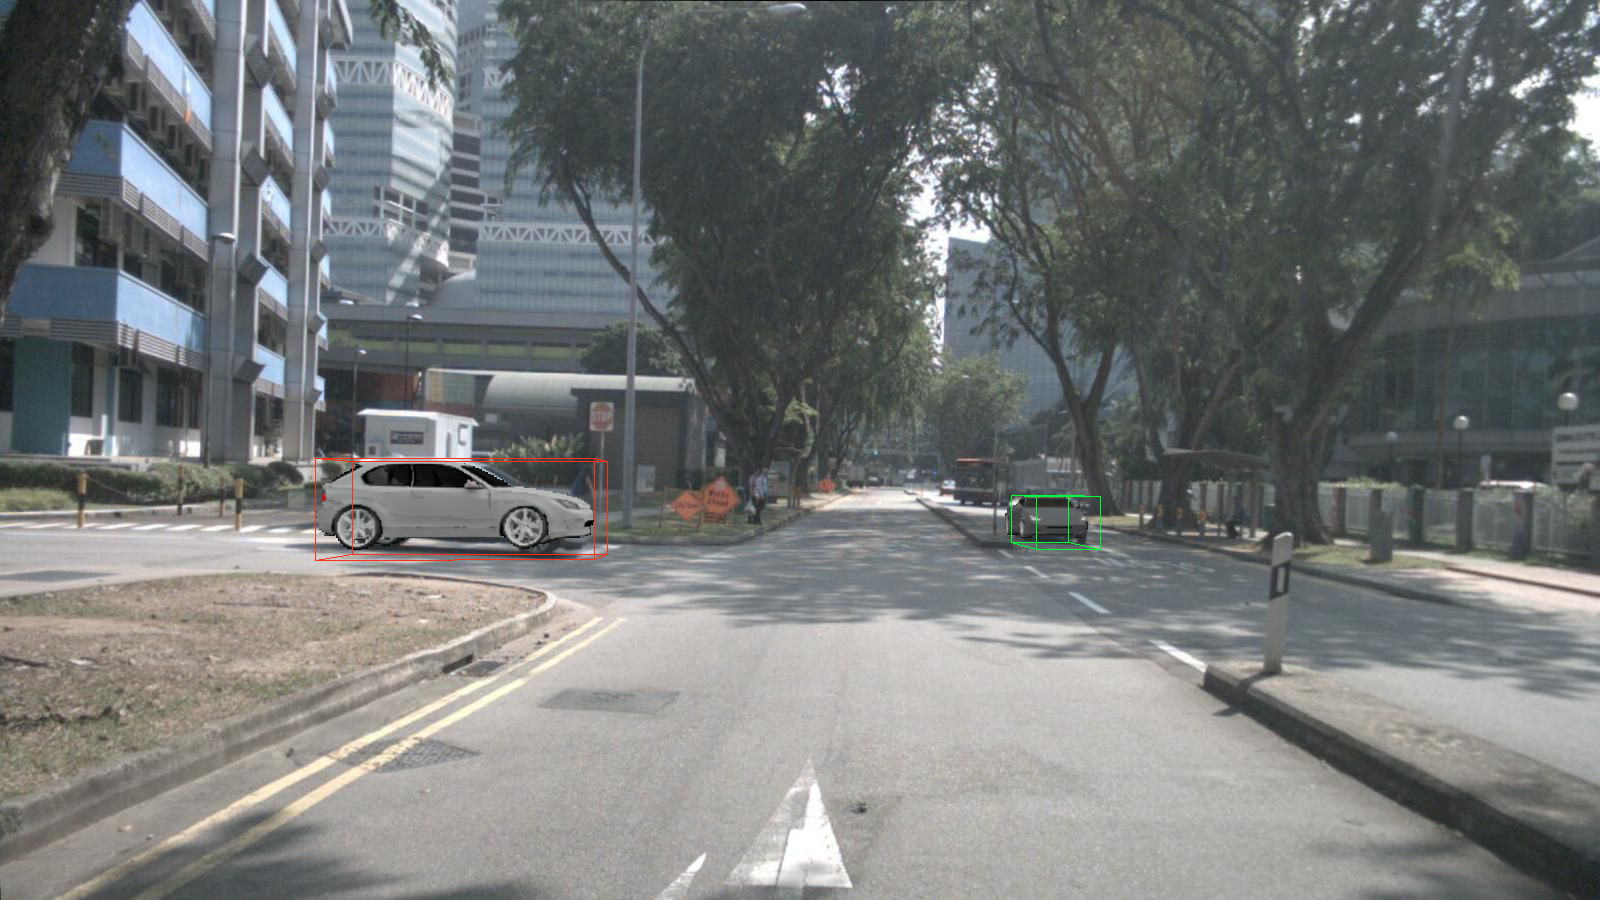
\includegraphics[width=.32\columnwidth, trim={0cm 0cm 0cm 0cm},clip]{fig/nuScenes_main/scene6/35_28_bbox.png}}&
		\raisebox{-0.5\height}{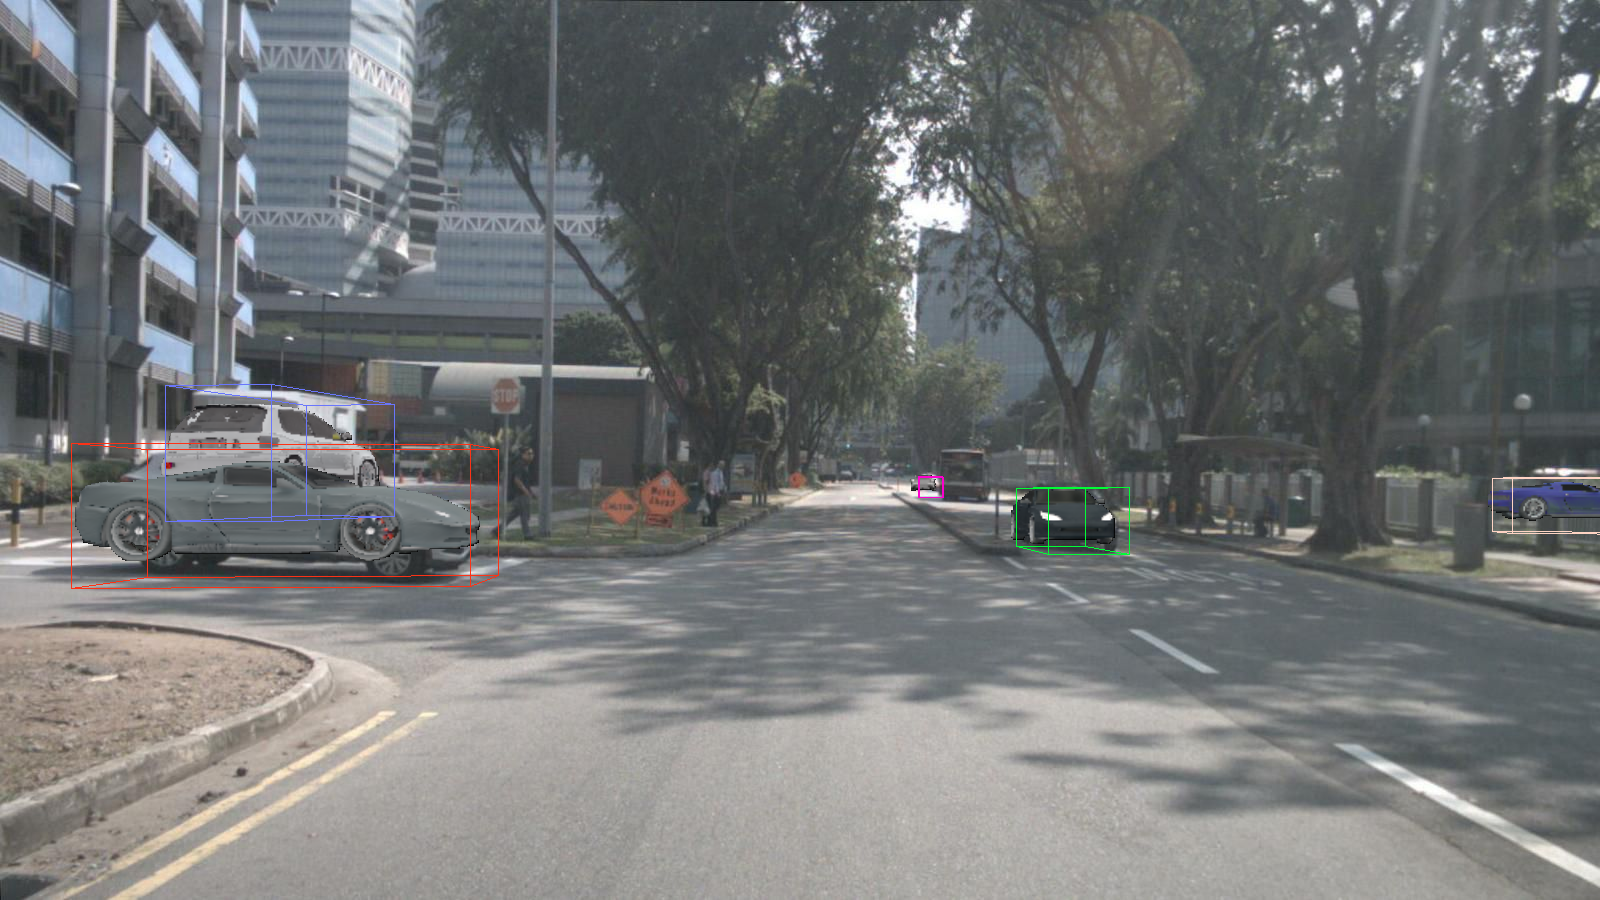
\includegraphics[width=.32\columnwidth, trim={0cm 0cm 0cm 0cm},clip]{fig/nuScenes_main/scene6/35_29_bbox.png}}&
		\raisebox{-0.5\height}{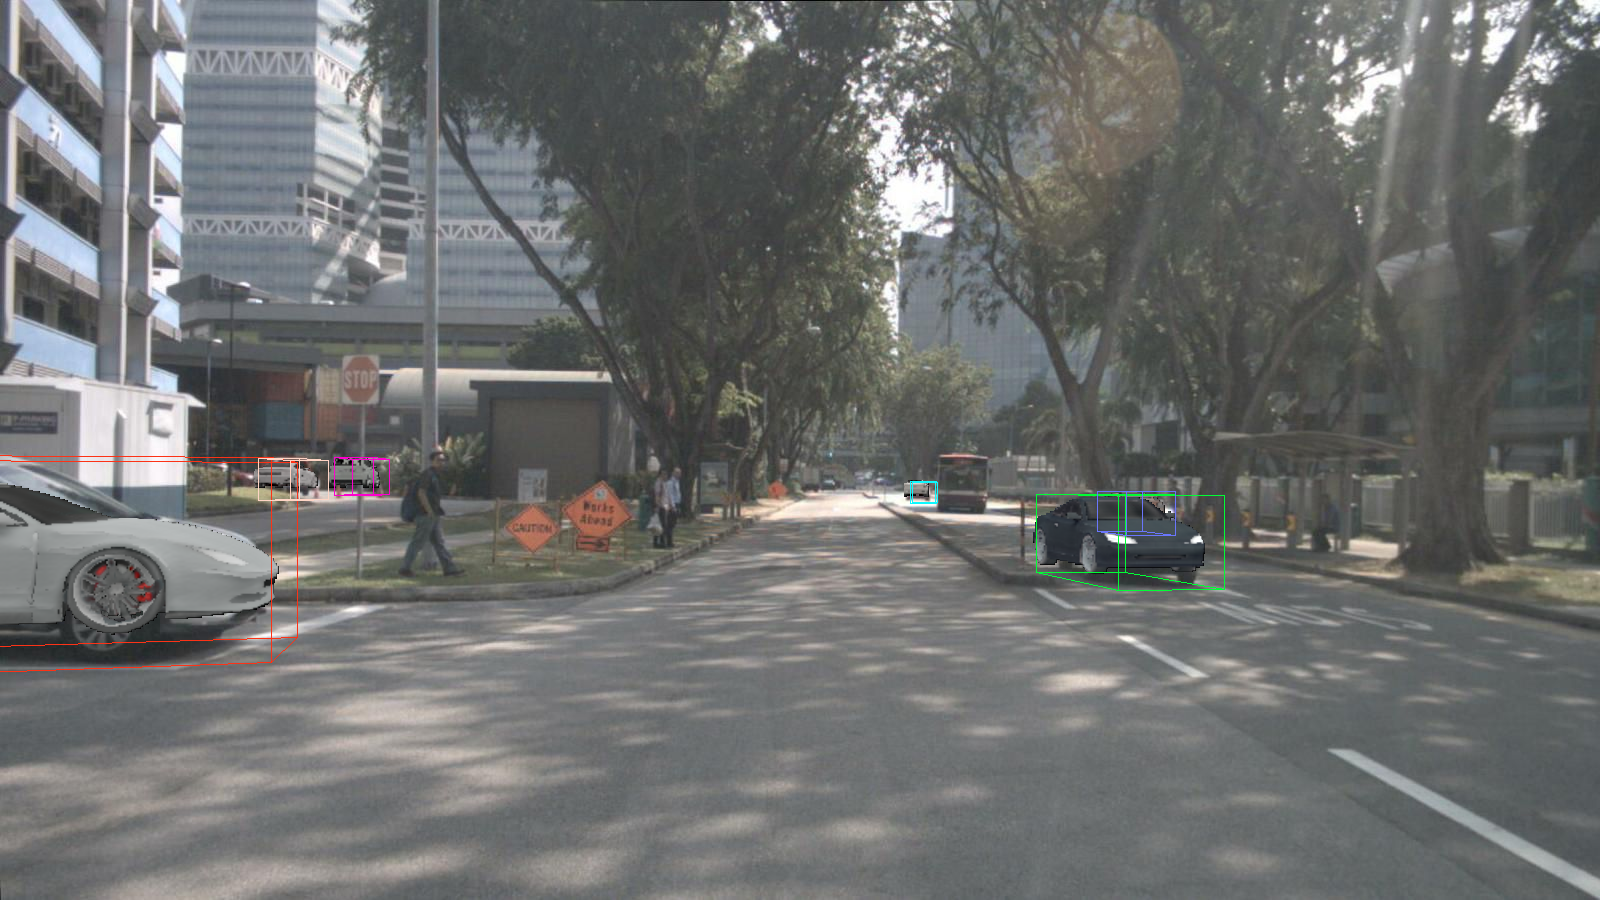
\includegraphics[width=.32\columnwidth, trim={0cm 0cm 0cm 0cm},clip]{fig/nuScenes_main/scene6/35_30_bbox.png}}&
		\raisebox{-0.5\height}{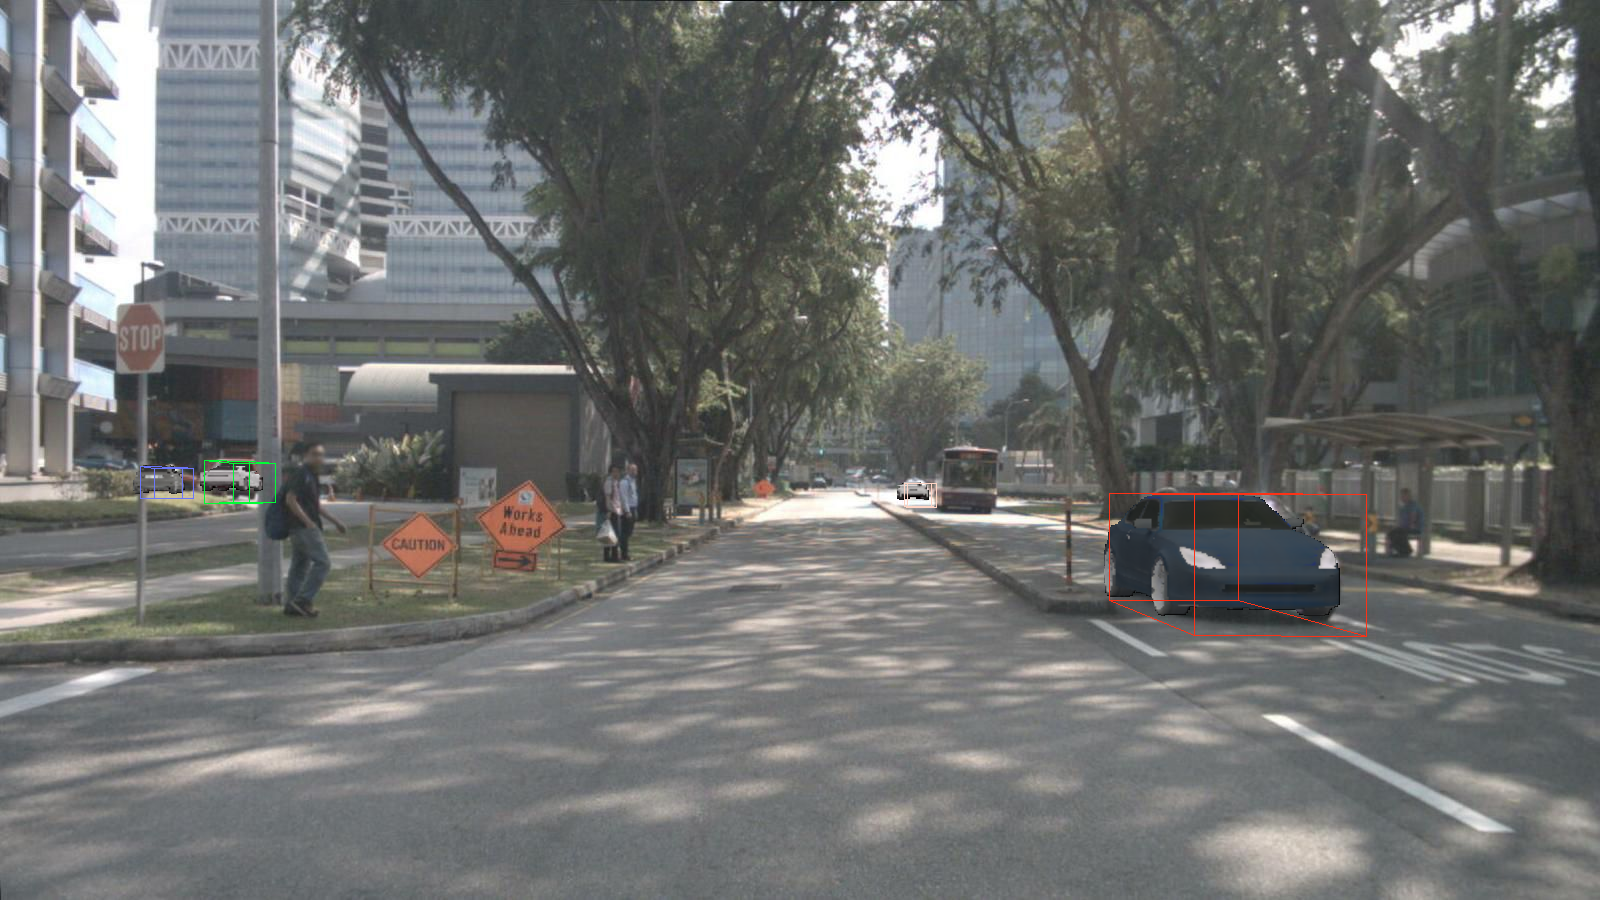
\includegraphics[width=.32\columnwidth, trim={0cm 0cm 0cm 0cm},clip]{fig/nuScenes_main/scene6/35_31_bbox.png}}\\[1.1cm]
  
            \rotatebox[origin=c]{90}{{\footnotesize	Parking lot}}&
  		\raisebox{-0.5\height}{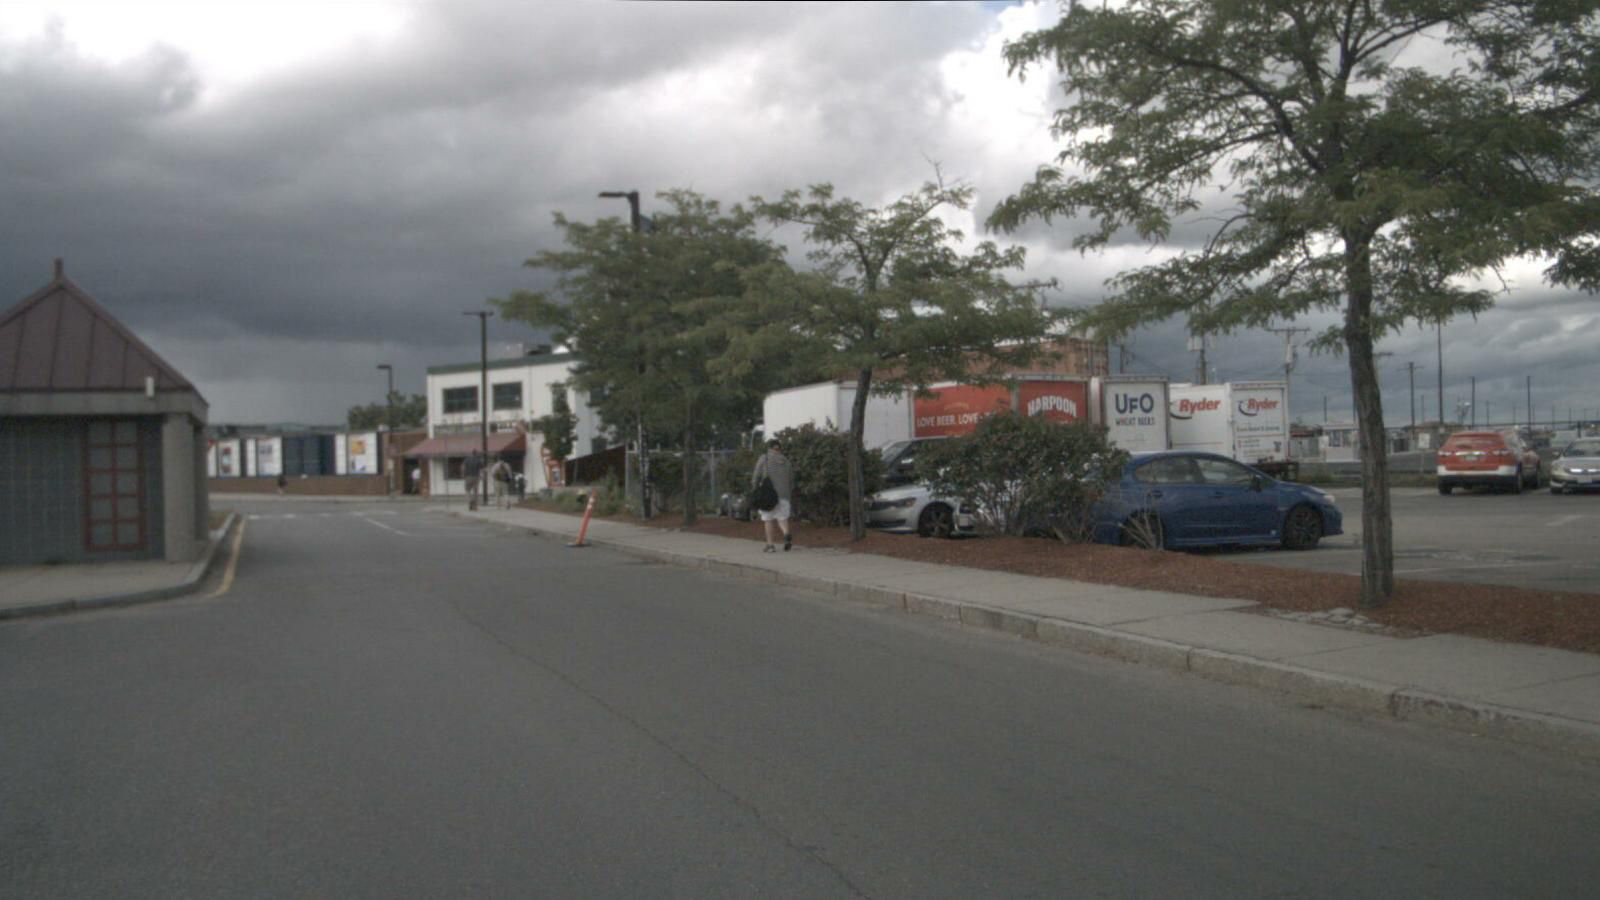
\includegraphics[width=.32\columnwidth, trim={0cm 0cm 0cm 0cm},clip]{fig/nuScenes_main/scene7/gt_2.png}}&
		\raisebox{-0.5\height}{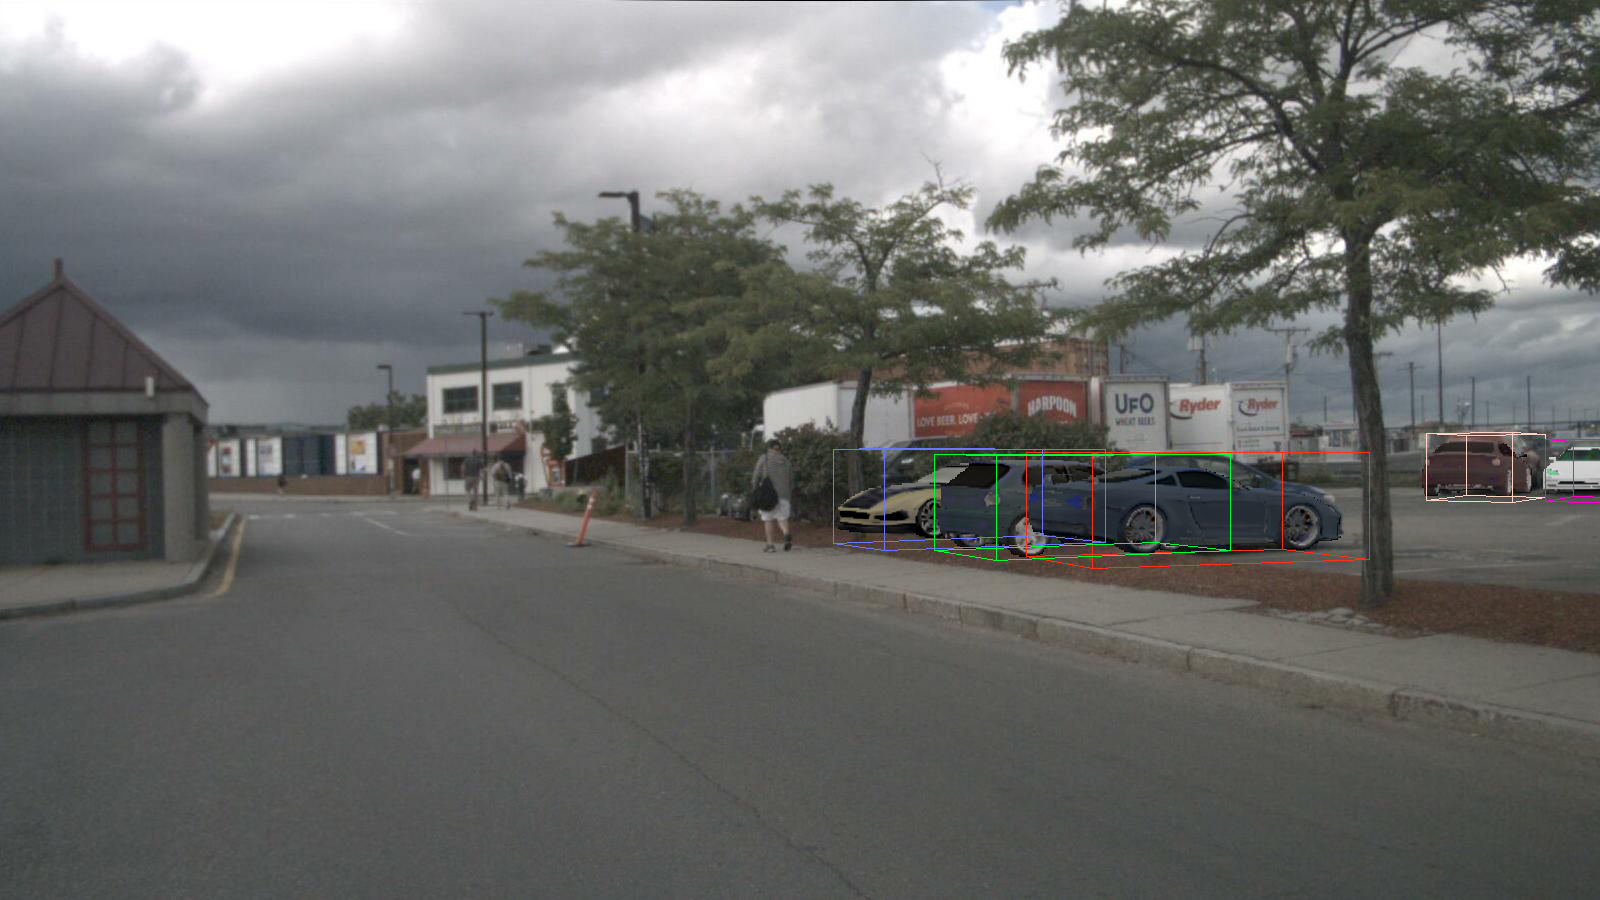
\includegraphics[width=.32\columnwidth, trim={0cm 0cm 0cm 0cm},clip]{fig/nuScenes_main/scene7/bbox_0.png}}&
		\raisebox{-0.5\height}{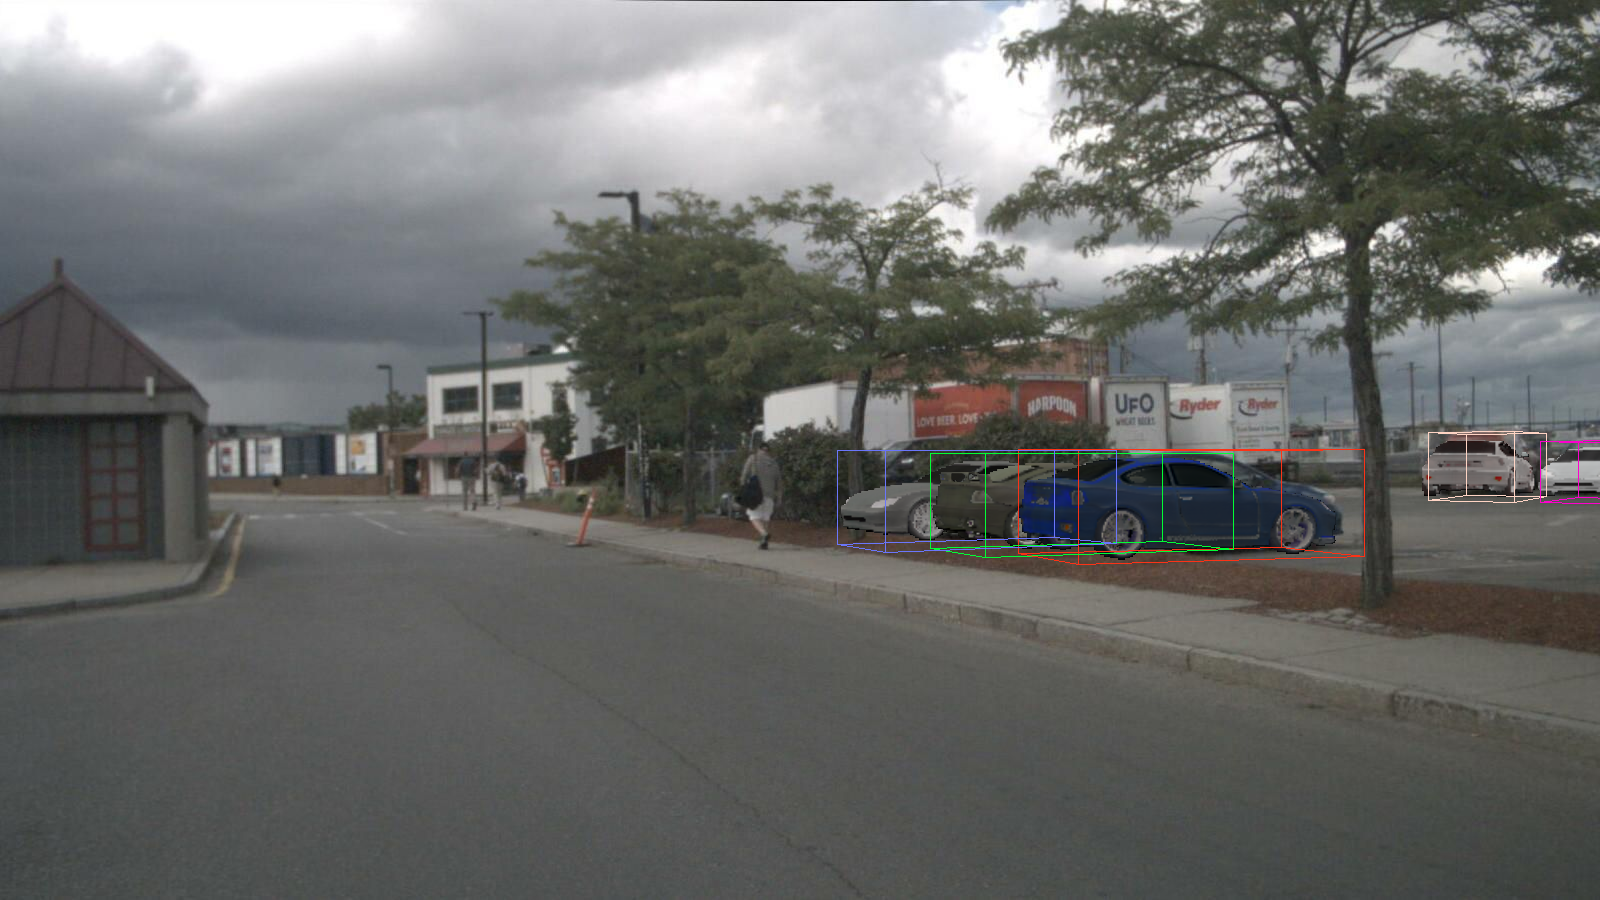
\includegraphics[width=.32\columnwidth, trim={0cm 0cm 0cm 0cm},clip]{fig/nuScenes_main/scene7/bbox_1.png}}&
		\raisebox{-0.5\height}{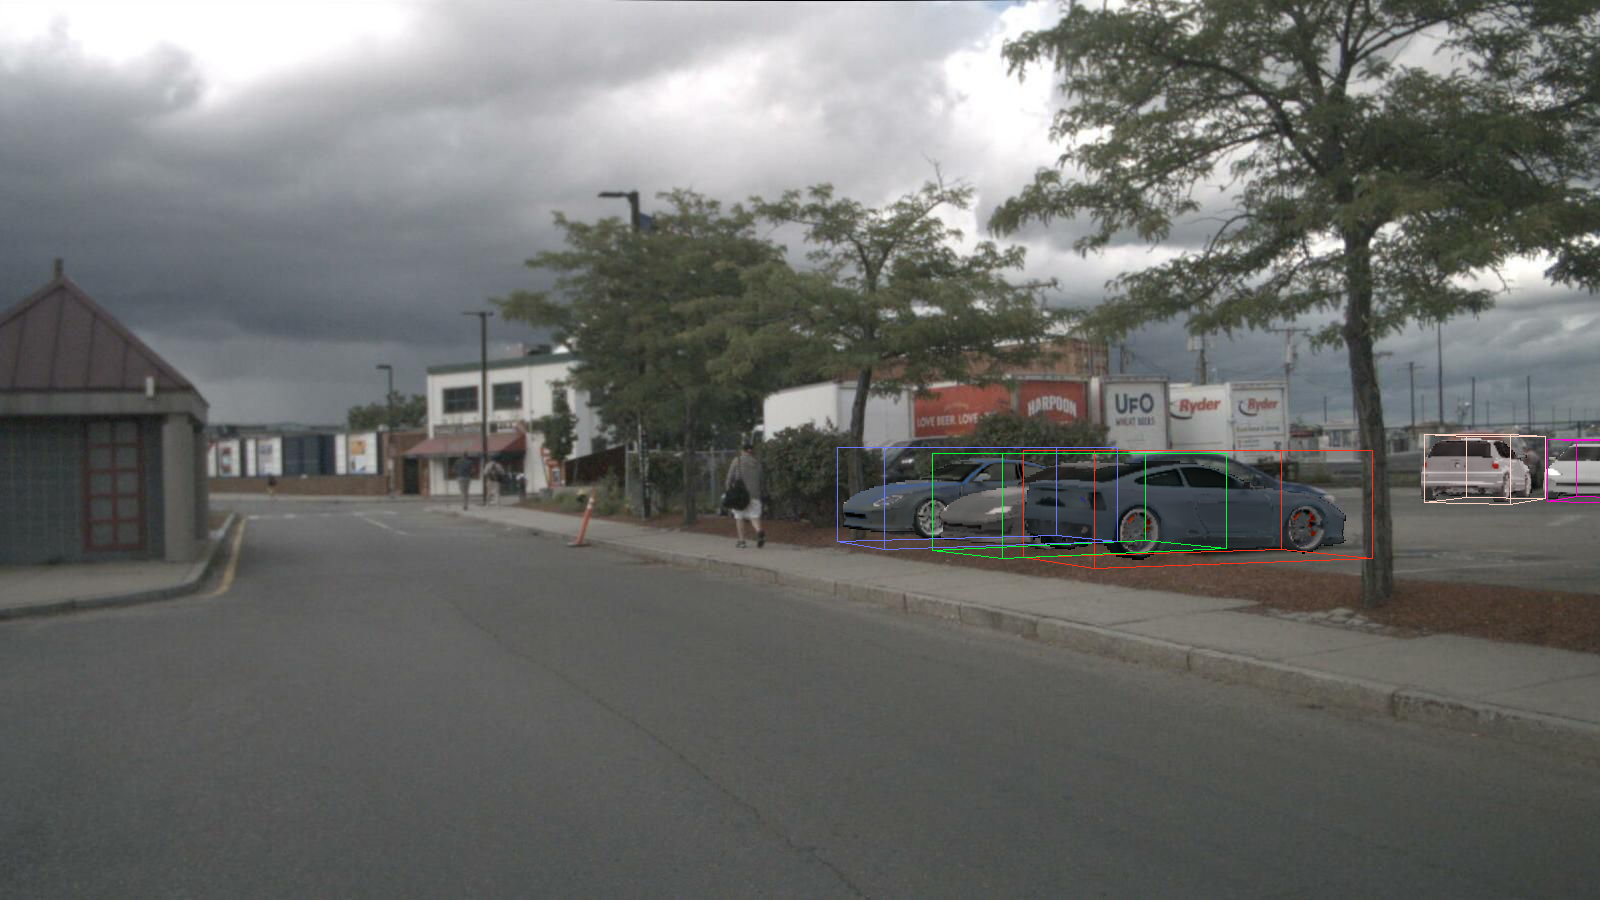
\includegraphics[width=.32\columnwidth, trim={0cm 0cm 0cm 0cm},clip]{fig/nuScenes_main/scene7/bbox_3.png}}&
		\raisebox{-0.5\height}{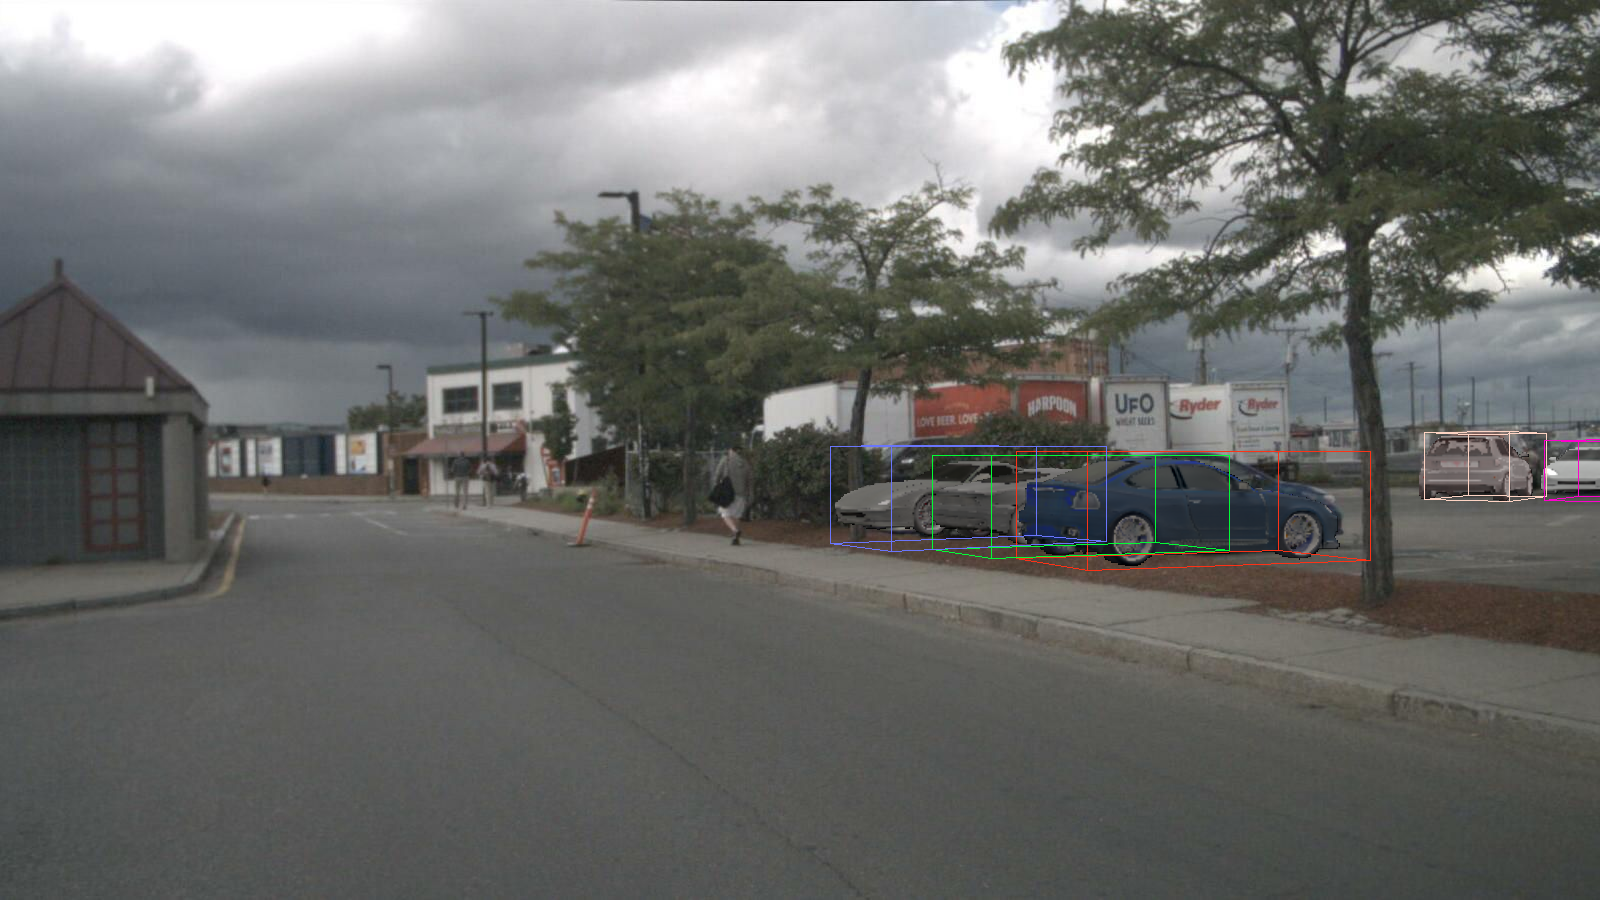
\includegraphics[width=.32\columnwidth, trim={0cm 0cm 0cm 0cm},clip]{fig/nuScenes_main/scene7/bbox_33.png}}\\%[0.95cm]
		
	\end{tabular}
	}
\vspace*{-6pt}
\caption{Tracking via Inverse Neural Rendering on nuScenes~\cite{caesar2020nuscenes}. From left to right, we show (i) observed images from diverse scenes at timestep $k=0$; (ii) an overlay of the optimized generated object and its 3D bounding boxes at timestep $k=0, 1, 2 \text{ and } 3$. The color of the bounding boxes for each object corresponds to the predicted tracklet ID. We see that even in such diverse scenarios, our method does not lose any tracks and performs robustly across all scenarios, although the dataset is unseen.}\label{fig:nuScenes_results}
\vspace*{-12pt}
\end{figure*}